\documentclass[10pt,fleqn]{article}

\usepackage[english]{babel}
\usepackage[utf8x]{inputenc}
\usepackage{enumerate}
\usepackage{amsmath}
\usepackage{amssymb}
\usepackage{amsfonts} 
\usepackage{mathtools}
\usepackage{graphicx}
\usepackage{bm}
\usepackage[usenames,dvipsnames]{color}
\usepackage{todonotes}
\usepackage{dsfont}
\usepackage{hyperref}
\hypersetup{
    colorlinks,
    citecolor=black,
    filecolor=black,
    linkcolor=black,
    urlcolor=black
}
\usepackage{algorithm}
\usepackage{algorithmic}
\usepackage{appendix}
\usepackage{subcaption}
\usepackage{fancyvrb}
\usepackage{subfigure}
\usepackage{graphicx,xcolor}
\usepackage{pifont,mdframed}
\usepackage{tikz}
\usepackage{bm}
\usetikzlibrary{fit,positioning}


%
% Macros
%
\newcommand \cashort[1] { {\todo[color=yello]{#1 -- Cedric}} }
\newcommand \calong[1]  { { \todo[inline,color=yellow]{#1 -- Cedric} } }
\newcommand \gbshort[1] { {\todo[color=cyan!40]{#1 -- Guillaume}} }
\newcommand \gblong[1]  { { \todo[inline, color=cyan!40]{#1 -- Guillaume} } }
\newcommand \mgshort[1] { {\todo{#1 -- Mark}} }
\newcommand \mglong[1]  { { \todo[inline]{#1 -- Mark} } }
\newcommand \bfshort[1] { {\todo[color=green!40]{#1 -- Bryan}} }
\newcommand \bflong[1]  { { \todo[inline,color=green!40]{#1 -- Bryan} } }


% Adds a plus const to the end of a math expression
\def \pcst{+\text{const}}

% A fancy version for capital R
\def \Rcal{\mathcal{R}}

% A fancy version for r
\def \rcal{\mathbf{r}}

% Loss function / log likelihood as appropriate
\def \L{\mathcal{L}}

% KL divergence [Math Mode]
\newcommand{\kl}[2] {
	\text{KL}\left[#1||#2\right]
}

\newcommand \vecf[1] {
    \text{vec}\left(#1\right)
}

\newcommand \ent[1] {
    \text{H} \left[ #1 \right]
}

\newcommand \mut[2] {
    \text{I} \left[ #1 ; #2 \right]
}

\newcommand \dvi[2] {
    \text{D}_\text{VI} \left[ #1; #2 \right]
}

% Starts an expected value expresses [Math Mode]
\newcommand{\starte}[1] {%
	\mathbb{E}_{#1}\left[
}

% Ends an expected value expression [Math Mode]
\def \ende{\right]}

% Starts an varianc expresses [Math Mode]
\newcommand{\startv}[1] {%
	\mathbb{V}\text{ar}_{#1}\left[
}

% Ends an variance expression [Math Mode]
\def \endv{\right]}

%\newcommand \ex[2] {
%    \bigl\langle #1 \bigr\rangle_{#2}
%}
\newcommand \ex[2] {
    \mathbb{E}_{ { #2 } }\left[ #1 \right]
}
\newcommand \var[2] {
    \mathbb{V}ar_{ { #2 } }\left[ #1 \right]
}

\newcommand \halve[1] {
	\frac{#1}{2}
}

\newcommand \half {
    \halve{1}
}

\newcommand \tr { \text{tr} } 

\newcommand \T { ^\top } 

\newcommand \fixme[1] {
    {\color{red} FIXME: #1}
}

\newcommand \vv[1] { \bm #1 }

\newcommand{\mbeq}{\overset{!}{=}}

\newcommand \diag[1] { \text{diag} \left( {#1} \right) }
\newcommand \diagonal[1] { \text{diagonal} \left( {#1} \right) }

\newcommand \Ed {{ \vv{\xi}_d}}
\newcommand \Edj {{\xi_{dj}}}
\newcommand \Edk {{\xi_{dk}}}
\newcommand \AEdj {{\Lambda(\xi_{dj})}}
\newcommand \AEdk {{\Lambda(\xi_{dk})}}
\newcommand \AEd  {{ \bm{\Lambda}(\bm{\xi}_d) }}

\newcommand \Axi { { \Lambda_{\xi} } }
\newcommand \bxi { { \vv{b}_{\xi} } }
\newcommand \cxi { { c_{\xi} } }


\newcommand \wdoc      { { \vv{w}_d } }
\newcommand \wdt[0]  { { w_{dt} } }
\newcommand \wdn[0]  { { \vv{w}_{dn} } }
\newcommand \wdnt[0]  { { w_{dnt} } }
\newcommand \wdd[0]   { { \vv w_{d} } }
\newcommand \zd[0]   { { \vv z_{d} } }
\newcommand \zdn[0]  { { \vv{z}_{dn} } }
\newcommand \zdnk[0] { { z_{dnk} } }
\newcommand \zdk[0]  { { z_{dk} } }
\newcommand \thd[0]  { { \vv \theta_d } }
\newcommand \thdk[0] { { \theta_{dk} } }
\newcommand \thdj[0] { { \theta_{dj} } }
\newcommand \epow[1] { { e^{#1} } }
\newcommand \pkt     { { \phi_{kt}  } }
\newcommand \pk      { { \vv \phi_k } }
\newcommand \lmd     { { \vv \lambda_d } }
\newcommand \lmdk    { { \lambda_{dk} } }
\newcommand \xd      { { \vv x_d } }
\newcommand \atxd     { A ^\top \bm x_d}
\newcommand \axd     { A\bm x_d}
\newcommand \tsq      { { \tau^2 } }
\newcommand \ssq      { { \sigma^2 } }
\newcommand \tmsq     { { \tau^{-2} } }
\newcommand \asq      { { \alpha^2 } }
\newcommand \amsq     { { \alpha^{-2} } }
\newcommand \sgsq     { { \sigma^2 } }
\newcommand \xvec     { { \vv{x} } }
\newcommand \omk      { { \bm \omega _k } }
\newcommand \omkt     { { \omega_{kt} } }
\newcommand \oma     { { \Omega_A } }
\newcommand \gdn      { { \vv{\gamma}_{dn} } }
\newcommand \gdnk     { { \gamma_{dnk} } }
\newcommand \gdk      { { \gamma_{dk} } }
\newcommand \isigt   { { \Sigma^{-1}_{\bm \theta} } }




\newcommand \halfSig { \frac{1}{2\sigma^2} }

\newcommand \nor[2]   { \mathcal{N} \left( {#1}, {#2} \right) }
\newcommand \nord[3]   { \mathcal{N}_{#1} \left( {#2}, {#3} \right) }
\newcommand \mnor[3]  { \mathcal{N} \left(#1, #2, #3\right) }
\newcommand \norp[3]  { \mathcal{N} \left(#1; #2, #3\right) }
\newcommand \mnorp[4] { \mathcal{N} \left(#1; #2, #3, #4\right) }
\newcommand \mul[1]   { \mathcal{M} \left( {#1} \right) }
\newcommand \muln[2]  { \mathcal{M} \left( {#1},{#2} \right) }
\newcommand \dir[1]   { \mathcal{D} \left( {#1} \right) }
\newcommand \pois[1]  { \mathcal{P} \left( {#1} \right) }
\newcommand \gp[2]    { \mathcal{GP} \left( {#1}, #2 \right) }
\newcommand \dir[1]   { \mathcal{D} \left( {#1} \right) }
\newcommand \gam[2]   { \mathcal{G} \left( {#1}, {#2} \right) }
\newcommand \beta[1]  { \mathcal{B}eta \left( {#1}, {#2} \right) }

\newcommand \lne[1]  { { \ln \left( 1 + e^{ #1 } \right) } }
\newcommand \Tr[1]   { \tr \left(  {#1}  \right) }

\newcommand \roud  { \vv{\rho}_{d}  }
\newcommand \rodk { \rho_{dk} }

\newcommand \exA[1]  { \ex{#1}{q(A)} }
\newcommand \exV[1]  { \ex{#1}{q(V)} }
\newcommand \exT[1]  { \ex{#1}{q(\Theta)} }
\newcommand \extd[1] { \ex{#1}{q(\thd)} }
\newcommand \exTV[1] { \ex{#1}{q(\Theta)q(V)} }

\newcommand \Real[0]  { { \mathbb{R} } }
\newcommand \VReal[1] { { \mathbb{R}^{#1} } }
\newcommand \MReal[2] { { \mathbb{R}^{#1 \times #2} } }
\newcommand \Nat[0]  { { \mathbb{N} } }
\newcommand \VNat[1] { { \mathbb{N}^{#1} } }
\newcommand \MNat[2] { { \mathbb{N}^{#1 \times #2} } }

\newcommand \inv[1] { {#1}^{-1} }
\newcommand \invb[1] { \inv{\left( #1 \right)} }

\newcommand \cn { \textsuperscript{\texttt{[{\color{blue}Citation Needed}]}} }

\newcommand \const { { \text{c} } }

\providecommand \floor [1] { \left \lfloor #1 \right \rfloor }
\providecommand \ceil [1] { \left \lceil #1 \right \rceil }


\newcommand \vt[2] { { #1^{(#2)} } }

\newcommand \hashtag[1] { { \ttfamily \##1 } }

\newcommand \mvy  { \vv{m}_{\vv{y}} }
\newcommand \sigvy { { S_Y } }

\newcommand \mmy  { M_Y      }
\newcommand \md   { \vv{m}_d }
\newcommand \phin { \vv{\phi}_n }
\newcommand \isigma { { \inv{\Sigma} } }

\newcommand \sigv     { { \Sigma_V } }
\newcommand \isigv     { { \Sigma^{-1}_V } }

\newcommand \sigy { { \Sigma_Y } }
\newcommand \isigy { { \Sigma_{-1}_Y } }


\newcommand \omy  { { \Omega_Y } }
\newcommand \iomy { { \inv{\Omega_Y} } }

\newcommand \siga     { { \Sigma_A } }
\newcommand \isiga     { { \Sigma^{-1}_A } }
\newcommand \diagv { { \diag{\nu_1,\ldots,\nu_P} } }

\newcommand \ma { \vv{m}_a }
\newcommand \my { \vv{m}_y }

\newcommand \VoU { V \otimes U }

\newcommand \one { \mathbb{1} }
%\newcommand \one  {{  \mathds{1} }}

\newcommand \lse { \text{lse} }
%\newcommand \lse[0] { \mathrm{lse} }

% Conditional independence 
\def\ci{\perp\!\!\!\perp} % from Wikipedia



% ------ For the eval section

% Multinomial PDF [Math Mode]
% params: 1 - the variable
%         2 - the value
%         3 - the state indicator (e.g. k for a distro with K values)
%         4 - any additional subscript
\newcommand{\mpdf}[4] {
	\prod_{#3} {#1}_{{#4} {#3}} ^ {#2}
}

% Dirichlet PDF [Math Mode]
% params: 1 - the variable
%         2 - the hyper-parameter
%         3 - the state indicator (e.g. k for a distro with K values)
%         4 - any additional subscript
\newcommand{\dpdf}[4] {
	\frac{1}{B({#2})} \prod_{#3} {#1}_{{#4} {#3}} ^ {({#2}_{#3} - 1)}
}

% To simplify the sampling equations, this is indicates
% that the given value has had datapoint "m" stripped out
%
\newcommand{\lm}[1] {
	#1^{\setminus m}
}

\newcommand \model[0] {
    \mathcal{M}
}

\newcommand \perplexity[1] {
    \mathcal{P} \left( { #1 } \right)
}

\newcommand \WTrain {
    \mathcal{W}^{(t)}
}

\newcommand \WQuery {
    \mathcal{W}^{(q)}
}

\newcommand \oneover[1] {
    \frac{1}{ {#1} }
}

\newcommand \samp[1] {
    { #1 }^{(s)}
}

\newcommand \etd[0] {
    \vv{\eta}_d
}

\begin{document}



\newcommand \xdn  { { \vv{x}_{dn} } }
\newcommand \zd   { { \vv{z}_d } }
\newcommand \qfam { { \mathcal{Q} } }
\newcommand \xdat { { \mathcal{X} } }
\newcommand \zdat { { \mathcal{Z} } }
\newcommand \xnew { { \vv{x}^{*} } }
\newcommand \znew { { \vv{z}^{*} } }
\newcommand \param { { \vv{\phi} } }
\newcommand \params { { \Phi } }
\newcommand \ml[1] { { {#1}_{\text{ML}} } } 
\newcommand \map[1] { { {#1}_{\text{MAP}} } } 
\newcommand \quarter { { \oneover{4} } }
\newcommand \eighth { { \oneover{8} } }
\newcommand \fqt[1] { { \mathcal{F}\left( {#1} \right) } }
\newcommand \joint { { p(\xdat, \zdat | \params) } }
\newcommand \logjoint { { \ln \joint } }
\newcommand \exlogjoint[1] { { \ex{\logjoint}{{#1}} } }

\chapter{Probabilistic Inference with Text}
This chapter reviews of probabilisitic inference from a Bayesian perspective. We introduce maximum-likelihood, maximum-a-posteriori, and fully Bayesian Inference. We describing inference schemes for latent variable models, and extend this to inference on large datasets using stochastic gradient descent (SGD), natural gradients, and biased sampling schemes. Finally, we provide a brief overview on Bayesian non-parametrics, and discuss the problem of evaluating model-fit.

Throughout, we use inference on text as a motivating example, and introduce language models, mixture-models of text, and admixture models of text, the last known colloquially as ``topic models". We quantitatively evaluate the effect that choices in models and inference schemes may have, and demonstrate the effect of different choices of evaluation metric.
\section{Inference Methods}

Probabilistic inference is concerned with two problems: inference, the estimation of parameter values $\param$ from a set of observations $\vv{x} \in \xdat$; and prediction, the evaluation of the probability of unobserved variables $p(\xnew | \xdat) = \int p(\xnew | \param) p(\param | \xdat) d\param$. Various methods have been proposed for this purpose.


\emph{Maximum likelihood} finds the parameter value that maximises, $p(\xdat|\param)$, known as the likelihood. For reasons of algebraic convenience\footnote{The log-likelihood can also be motivated by Information Theory. Since mean negative log-likelihood asymptotically converges to the Shannon-Entropy, minimising it leads to a model that better ``compresses" data. This idea is discussed in detail in \cite{MacKay2005InfoTheory} }, one commonly finds the maximum of the log of the likelihood.

% For MLE / Info Theory: https://quantivity.wordpress.com/2011/05/23/why-minimize-negative-log-likelihood/
% http://thirdorderscientist.org/homoclinic-orbit/2013/4/1/maximum-likelihood-and-entropy
\begin{align}
\ml{\param} = \arg \max_{\param} \ln p(\xdat | \param)
\end{align}

As the log of a monotonically increasing function, the log-likelihood and likelihood have the same maxima. For the particular case of independently and identically distributed (IID) observations, the log-likelihood factors into a simple sum.

\begin{align}
\ml{\param} = \arg \max_{\param} \sum_d \ln p(\xd | \param) \label{eqn:log-like-iid-decomp}
\end{align}


For prediction one typically employs the approximation

\begin{align}
p(\xnew | \xdat) 
&= \int p(\xnew | \param) p(\param | \xdat) d\param \label{eqn:ml-prediction}\\
&\approx \int p(\xnew | \ml{\param}) p(\param | \xdat) d\param
=  p(\xnew | \ml{\param})
\end{align}

The same decomposition used in \eqref{eqn:log-like-iid-decomp} can also be derived from the assumption that the data are \emph{exchangeable}.  A finite sequence of random variables $\xdat = \{\xd\}_{d=1}^{D}$ is exchangeable if its joint distribution is invariant to any permutation of its order. An infinite sequence is exchangeable, if all finite subsequences are themselves exchangeable. The link with IID observations is provided by DeFinetti's theorem (extended to the multinomial case\bfshort{What is the ``multinomial case"} in \cite{Hewitt1955}) which states that the joint distribution of an exchangeable sequence of variables is equivalent to sampling a random parameter $\param$ from some prior distribution, then sampling IID random variables conditional on that random parameter such that $p\left(\xdat\right) = \prod_d p(\xd | \param)$.

\emph{Maximum a Posteriori} (MAP) estimation, like maximum likelihood, finds a mode, but of the posterior distribution instead of the likelihood. Given a prior $p(\param)$, the posterior is given by Bayes rule:
\begin{align}
p(\param | \xdat) = \frac{p(\xdat | \param)p(\param)}{p(\xdat)} = \frac{\text{likelihood} \times \text{prior}}{\text{evidence}}
\end{align}

The MAP solution is:

\begin{align}
\map{\param} = \arg \max_{\param} \frac{p(\xdat | \param)p(\param)}{p(\xdat)}
 & = \arg \max_{\param} p(\xdat | \param)p(\param) \\
 & = \arg \max_\param \ln p(\xdat | \param) + \ln p(\param)
\end{align}
Prediction follows similarly to ML
\begin{align}
p(\xnew | \xdat) \approx \int p(\xnew | \map{\param})p(\param|\xdat)d\param = p(\xnew | \map{\param})
\end{align}



The incorporation of the prior is motivated by two related reasons: firstly it allows a practitioner to supply some prior knowledge to the inference procedure and secondly it prevents a model from overfitting in the presence of limited or noisy data.

The alternative to finding modes is to take a fully \emph{Bayesian} approach, solve Bayes rule directly, and thereby derive a \emph{distribution} over $\param$. This in turn means we can evaluate our predictions exactly, by solving the integral \eqref{eqn:ml-prediction} and thereby get a measure of the uncertainty in our predictions.

The Bayesian approach involves evaluating the evidence $p(\xdat) = \int p(\xdat | \param) p(\param) d\param$. In many cases this is intractable, but there are families of prior and likelihood distributions where the prior and posterior have the same functional form for which exact inference is possible. In these cases we say the prior is \emph{conjugate} to the likelihood.

\begin{figure}
  \centering
    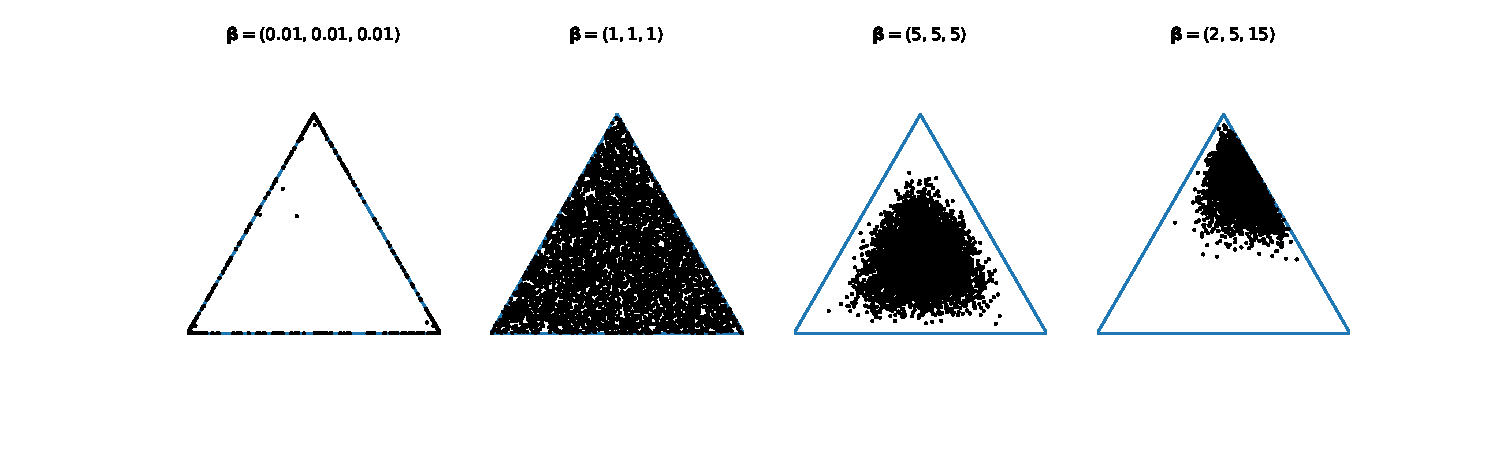
\includegraphics[width=0.97\textwidth]{../Chap1/plots/dirichlet_samples.pdf}
  \caption{Samples drawn from a three-dimensional Dirichlet distribution parameterised by different vectors $\vv{\beta}$. Observe that these 3D samples exist on a 2D simplex.}
  \label{fig:dirichlet-params}
\end{figure}

An example is learning a parameter $\param$ with a Dirichlet distribution given multinomial-distributed observations (e.g. throws of a weighted dice). The Dirichlet distribution is given by:
\begin{align}
p(\param) & = \oneover{B(\vv{\beta})} \prod_k \phi_k^{(\beta_k - 1)} &
B(\vv{\beta}) & = \frac{\prod_k \Gamma(\beta_k)}{\Gamma(\sum_k \beta_k)}
\end{align}
where $B(\cdot)$ is the multivariate beta function, and $\Gamma(\beta)$ is the Gamma function, which can be thought of as a continuous generalisation of the factorial function such that $x! = \Gamma(x+1)$. The multinomial is given by:
\begin{align}
p(\vv{x}|\param) = \frac{(\sum_k x_k)!}{\prod_k x_k!} \prod_k \phi_k^{x_k}
\end{align}
though for a single draw, the  quotient evaluates to one. A single-draw multinomial distribution is known as a \emph{categorical} distribution, and will be denoted in this thesis with the notation $\vv{x}|\param \sim \cat{\param}$. The joint distribution of several, exchangeable observations using a categorical likelihood is 
\begin{align}
p(\xdat|\param) & = \prod_d \prod_k \phi_k^{x_{dk}} = \prod_k \phi_k^{n_k} &
n_k = \sum_d x_{dk}
\end{align}
Using this we can analytically evaluate the evidence $p(\xdat)$:
\begin{align}
p(\xdat) & = \frac{1}{B(\beta)} \int \prod_k \phi_k^{n_k} \prod_k \phi_k^{(\beta_k - 1)} d\param  = \frac{1}{B(\beta)} \int \prod_k \phi_k^{n_k + \beta_k - 1} \\
& = \frac{B(\vv{n} + \vv{\beta})}{B(\vv{\beta})} \label{eqn:polya-is-evidence}
\end{align}
The analytic solution arises from observing that the integrand is an unnormalised Dirichlet distribution parameterised by $\vv{n} + \vv{\beta}$ where $\vv{n} = \{ n_k \}_{k=1}^K$. This marginal distribution is sometimes known as the P\'{o}lya distribution, or the Dirichlet-compound-Multinomial distribution \cite{Madsen2005}.\label{polya}

Putting this together we can analytically derive an expression for the posterior:

\begin{align}
\begin{split}
p(\phi|\xdat) 
& = \frac{p(\phi|\xdat)p(\phi)}{p(\xdat)}
 = \left(\prod_k \phi_k^{n_k} \right)
   \left(\oneover{B(\vv{\beta})} \prod_k \phi_k^{\beta_k - 1} \right)
   \frac{B(\vv{\beta})}{B(\vv{n} + \vv{\beta})} \\
& = \oneover{B(\vv{n} + \vv{\beta})} \prod_k \phi_k^{n_k + \beta_k - 1}
\end{split}
\end{align}
which is a Dirichlet distribution parameterised by $\vv{n} + \vv{\beta}$

It is useful to compare the expected value of the posterior with the MAP and maximum likelihood solutions.

\begin{align}
\ex{\phi_k}{}  &= \frac{n_k + \beta_k}{\sum_j n_j + \beta_j} &
\phi_k^{\text{MAP}} &= \frac{n_k + \beta_k - 1}{\sum_j n_j + \beta_j - 1} &
\phi_k^{\text{ML}}  &= \frac{n_k}{\sum_j n_j}
\end{align}

The Bayesian approach is more affected by the prior than the MAP solution, where the prior is discounted, and the ML approach obviously incorporates no prior information whatsoever. 

\subsubsection*{A Note on Categorical and Multinomial Distributions}
In this thesis, we will frequently posit models where we sample words one at a time. 

One representation of this is to use a scalar $x \in \{1 \ldots T\}$ whose value indicates the word chosen. This gives rise to a \emph{categorical} distribution parameterised by a vector $\vv{\phi} \in \VReal{T}$
\begin{align}
x &\sim \cat{\vv{\phi}}&
p(x) = \prod_t \phi_t^{[x = i]}
\end{align}
where $[x = i]$ is the Iverson bracket -- an extension of the Dirac delta -- which evaluates to 1 if the condition is true, and zero otherwise. 

An equivalent representation is a 1-of-T vector $\vv{x}$, where all elements are set to zero except one which is set to 1, one whose index indicates the word chosen. This gives rise to a multinomial distribution parameterised by a vector $\vv{\phi} \in \VReal{T}$ for which the number of trials is fixed at 1.
\begin{align}
\vv{x} &\sim \muln{\vv{\phi}}{1} &
p(x) = \frac{1!}{\prod_t x_t!}\prod_t \phi_t^{x_t} = \prod_t \phi_t^{x_t}
\end{align}
In all cases in this thesis, when we say a variable has a \emph{categorical distribution}, we mean to say it is a 1-of-T vector with a multinomial distribution for which the number of trials is fixed at one. Depending on context we may refer to it as a 1-of-T vector or as a categorical scalar. 

 
\subsection*{Example: Language Models}
 \label{sec:chap1:mackay-lang-model}
An example of conjugate inference is the language-modelling problem. This is the problem of predicting the next word in a sequence of discrete observations from a finite vocabulary (e.g a sentence) given all previous observations. Common use-cases are predictive keyboards, spell-checkers and speech recognition.\bfshort{Cite use-cases}

As vocabularies are normally quite large (typically of the order of 30,000 terms), raising this to the power of two or three can lead to models that are over-parameterised: in particular maximum likelihood estimates will often collapse to zero in the absence of training data. ``Laplace smoothing", equivalent to MAP inference using a symmetric Dirichlet prior, is a simple remedy, but unsatisfying in that it does not take into account the information available in the lower-order n-grams.

Using conjugate Bayesian inference it is possible to create a first-order (i.e. bigram) language model\cite{MacKay1995} that uses unigram statistics. Given a sequence of observations $x_1, \ldots, x_D$, where each $x_d \in \{1 \ldots T\}$, we can define for each of the $T$ words a distribution over the next possible word $\vv{\phi}_t \in \VReal{T}$.

\begin{align}
x_i | x_{i - 1} 
& \sim \cat{\vv{\phi}_{x_{i-1}}}
& \vv{\phi}_t 
& \sim \dir{\vv{\beta}}
\end{align}

As before, used a corpus W to estimate our parameters, the \emph{exact} predictive distribution is
\begin{align}
p(w_i = t | w_{i-1}, W)
& = \ex{\phi_{w_{i-1},t}}{}
  = \frac{n_{w_{i-1},t} + \beta_t}{\sum_v n_{w_{i-1},v} + \beta_v}
\end{align}
where $n_{w_{i-1},t}$ denotes the number of times value $t$ was observed immediately after the value of $w_{i-1}$. The preceding sequence (in this case a single term) is known as the \emph{context}

Since the prior term $\beta_v$ will occur in all contexts, one can incorporate unigram probabilities in our bigram estimates by learning the prior $\vv{\beta}$. This approach, of sharing information between contexts in an inference task, is sometimes known as \emph{multi-task learning} and will be discussed in detail in Chapter 3.

Marginalising out the parameters $\vv{\phi}_t$ provides the model evidence $p(W|\vv{\beta})$ as in equation \eqref{eqn:polya-is-evidence}. The derivative of this with respect to $\beta_v$ is:
\begin{align}
\frac{d \ln p(W|\vv{\beta})}{d\beta_v} =
\sum_t
     \Psi(\sum_u \beta_u) 
     - \Psi(n_{\cdot|t} + \sum_u \beta_u)
     + \Psi(n_{v|t} + \beta_v)
     - \Psi(\beta_v)
\end{align}
where $n_{v|t}$ is the number of times word $v$ has been seen after word $t$ and $n_{\cdot|t} = \sum_v n_{v|t}$. The digamma function $\Psi(\cdot)$ is the derivative of the gamma function $\Gamma(\cdot)$. This leads to a simple re-estimation method for $\beta_v$

\begin{align}
\beta^{new}_v = \beta_v \frac{
        \sum_t \Psi(n_{v|t} + \beta_v) - \Psi(\beta_v)
    }{
        \sum_t \Psi(n_{\cdot|t} + \sum_u \beta_u) - \Psi(\sum_u \beta_u)
    }
\end{align}


There are in fact a variety of methods of inferring a Dirichlet distribution, which are explored more fully in \cite{Minka2000}. For example, taking the fully Bayesian perspective, one might want to regulate inference over $\vv{\beta}$ by putting priors on it in turn. In this case it's useful to reformulate the Dirichlet as being parameterised by a concentration parameter $\beta$ with a Gamma prior and a base measure $\vv{u}$ on the simplex with a symmetric Dirichlet prior, such that $\vv{\phi}_t  \sim \dir{\beta \cdot \vv{u}}$.


This Bayesian model builds on the frequentist Jelinek Mercer\cite{JelinekMercer1980} interpolated language model, wherein the probability of an n-gram was a weighted combination of the probabilities of all m-grams for $m \in \{n, (n-1), \ldots, 1\}$. So for a bigram $p(w_i|w_{i-1}) = \lambda p(w_i|w_{i-1}) + (1 - \lambda) p(w_i)$. Jelinek Mercer required different $\lambda$ for each distinct context (sequence of words $w^i_{i-n+1}$), learned through cross-validation. By contrast, the Baysesian perspective leads to a model that neatly balances between the two based on the number of bigram and unigram observations.

An alternative to interpolation models are ``back-off" language-models. One ``backs off" to a simpler estimate if no data exists to support a higher order estimate, i.e the n-gram count is zero. Back-off models typically use a form of discounting, removing a portion of counts from frequently occurring n-grams and assigning the resultant spare probability mass to lower-order n-grams. The best performing back-off model is Knesser-Ney \cite{Chen1999} , which defines the probability of a word as 
\begin{align}
p_\text{KN}(w_i | w^{i-1}_{i-n+1}) = \left\{ \begin{array}{lr}
     \frac{\max\{c(w^i_{i-n+1}) - D, 0\}}{\sum_{w_i} c(w^i_{i-n+1})} & \text{if } c(w_i, w_{i-1}) > 0 \\
     \lambda(w^{i-1}_{i-n+1}) p_\text{KN}(w_i | w^{i-1}_{i-n+2}) & \text{otherwise}
 \end{array}
\right.
\end{align}
where $c(\cdot)$ denotes the count of how often the word sequence was observed in the data. In order to accumulate enough probability mass to assign to the unobserved n-grams, mass is ``skimmed" off the observed n-grams using the discount term $D$. This is then used in the normalisation term $\lambda(w^{i-1}_{i-n+1}) = \frac{D}{\sum_{w_i} c(w^{i-1}_{i-n+1})}$ which ensures all probabilities sum to 1. The value of $D$ is normally found using cross validation.

One can augment back-off models with interpolation. An interpolated variant of Knesser-Ney called ``modified Knesser-Ney"\cite{Chen1999} is one of the best performing language models currently in use, and performs better than the Bayesian approach described above\cite{Teh2002}. This is defined as

\begin{align}
\begin{split}
p_\text{KN}(w_i | w^{i-1}_{i-n+1}) & = 
\frac{\max\{c(w^i_{i-n+1}) - D, 0\}}{\sum_{w_i} c(w^i_{i-n+1})} \\
& + \lambda(w^{i-1}_{i-n+1}) N_{1+}(w^{i-1}_{i-n+1}, *) p_\text{KN}(w_i | w^{i-1}_{i-n+2})
\end{split}
\end{align}
where $N_{1+}(w^{i}_{i-n}, *)$ is the number of unique contexts (i.e. prefixes) in which the n-gram $w^{i}_{i-n}$ has occurred.  This is a unique feature of interpolated Knesser-Ney: given the sentence ``He left San Francisco via San Francisco airport" a higher unigram probability will be assigned to ``San" as it occurs in two contexts (``left" and ``via") than ``Francisco" which only occurs after ``San". Later in this chapter we will introduce a probabilistic alternative to Knesser-Nye when discussing non-parametric Bayesian methods\bfshort{Follow up on this}

A further discussion of language-modeling -- including other interpolation and backoff models such as Katz-Smoothing, Witten-Bell Smoothing, Good-Turing Estimation and Absolute Discounting -- is provided by \cite{Goodman2001}.


 
\section{Latent Variable Models}
Oftentimes it is appropriate to assume that there is some unobserved, latent process which determines the distributions of the observed variables. Denoting the latent variables as $\zdat$ this gives rise to the following likelihood
\begin{align}
p(\xdat|\params) = \int p(\xdat, \zdat|\params) d\zdat
\end{align}

A common case where latent variables arise is the mixture model, where it is assumed there are $K$ distributions, of which one, identified by a latent categorical variable $\vv{z}_d$ is used to sample an observation $\xd$. 

Our MAP solution is
\begin{align}
\begin{split}
\params 
    &= \arg \max_\params \ln p(\params) + \ln p(\xdat|\params) \\
    &= \arg \max_\params \ln p(\params) + \ln \int \joint d\zdat \label{eqn:em-problem}
\end{split}
\end{align}

In this case of a mixture model, since mixture assignments $\vv{z}_d$ have a categorical distribution
\begin{align}
\ln \int \joint d\zdat = \ln \left(\sum_Z \joint\right)
\end{align}

In many cases either the integral in \eqref{eqn:em-problem} has no analytic solution, or evaluating it is simply not tractable. In this case one uses an approximation, leading to the Expectation-Maximisation algorithm.
\subsection{Expectation Maximisation}
Jensen's inequality states that for any \emph{concave} function $f(x)$, $f\left(\ex{x}{}\right) \geq \ex{f(x)}{}$. By introducing an arbitrary distribution $q(\zdat)$ over the latent variables, we can employ the inequality to approximate log-integral in equation \eqref{eqn:em-problem}

\begin{align}
 \ln p(\xdat|\params) & = \ln \int \joint d\zdat =  \ln \int \frac{q(\zdat)}{q(\zdat)} \joint d\zdat\\ 
     &=  \ln \ex{\oneover{q(\zdat)}\joint}{q} \geq  \ex{\ln \oneover{q(\zdat)}\joint}{q}\\
     &= \ex{\ln \joint}{q} + \ent{q} \label{eqn:elbo}
\end{align}
where the entropy $\ent{q} = -\ex{\ln q(\zdat)}{q}$. Equation \eqref{eqn:elbo} is sometimes referred to as the \emph{free energy} or the \emph{evidence lower-bound} (``ELBO").

This leads two a two-step, iterative, maximisation process, where at each iteration $i$ we first find the distribution over our latent variables that maximises the ELBO, and then secondly use that to approximate the integral and find the distribution over our parameters that maximise the likelihood.

\begin{align}
\text{E-Step:} & & q^i(\zdat) & = \arg \max_{q(\zdat)} \ex{\ln p(\xdat, \zdat|\params^{i-1})}{q^{i-1}} + \ent{q} \label{eqn:estep} \\
\text{M-Step:} & & \params^i & = \arg \max_{\params} \ex{\ln \joint}{q^{i}} + \ln p(\params) \label{eqn:mstep}
\end{align}
To determine how to maximise $q(\zdat)$ we observe that, for a fixed $\params$, the difference between the ELBO and the marginal log-likelihood is given by
 the Kullback Leibler divergence between $q(\zdat)$ and the posterior $p(\zdat|\xdat, \params)$.
\begin{align}
\int q(\zdat) \ln \frac{p(\xdat, \zdat|\params)}{q(\zdat)} d\zdat
& = \int q(\zdat) \ln \frac{p(\zdat|\xdat, \params)p(\xdat | \params)}{q(\zdat)} d\zdat \\
& = \int q(\zdat) \ln p(\xdat | \params) q\zdat + \int q(\zdat)\ln\frac{p(\zdat|\xdat, \params)}{q(\zdat)} d\zdat \\
& = \ln p(\xdat | \params) + \kl{q(\zdat)}{p(\zdat|\xdat, \params)}
\end{align}
As the Kullback-Leibler divergence is always positive, reducing the divergence will increase the ELBO. Its maximum, $\ln p(\xdat | \params)$, is attained when $\kl{q(\zdat)}{p(\zdat|\xdat, \params)} = 0$. Therefore the  E-Step maximisation step is to set $q(\zdat) = p(\zdat | \xdat, \param)$.

This is the MAP variant of the Expectation Maximization (EM) algorithm\cite{Dempster1977}. 
Both E and M steps increase the bound. In the M-Step, we maximise the ELBO with respect to $\params$, increasing both the likelihood and the ELBO. In the E-Step by setting $q(\zdat) = p(\xdat|\zdat, \params)$ the KL divergence goes to zero, decreasing the gap between the ELBO and marginal likelihood. Consequently EM is guaranteed to find a local maximum of the marginal likelihood.\bfshort{Reference for convergence}

\subsection*{Example: A Mixture of Multinomials}
\label{sec:ch1:mom}
\bflong{Add Poisson to Multinomial Here}
As an example, consider the problem of modelling a corpus of documents. Let $\xd \in \mathbb{N}^T$ be the count of how often each word occurred in document $d$, for all $T$ words (known as the bag-of-words model). If we presume each document is about one of K topics, where each topic has a distribution over word-counts $\vv{\phi}_k$, we can associate a latent categorical variable $\vv{z}_d$ with each document indicating which (unobserved) topic generated its words. Denoting document d's word-count as $n_d = \sum_t x_{dt}$, and letting $\params = \{ \vv{\phi}_{k=1}^K \}$, this gives rise to the mixture of multinomials model\cite{Nigam2000}
\begin{align}
\vv{\theta} & \sim \dir{\vv{\alpha}} &
\zd|\vv{\theta} & \sim \muln{\vv{\theta}}{1} & 
\xd|\zd, \params & \sim \prod_k \muln{\param_k}{n_d}^{z_{dk}} & 
\param_k & \sim \dir{\vv{\beta}}
\end{align}
Note that in this model the Dirichlet hyper-parameters $\vv{\alpha}$ and $\vv{\beta}$ are coupled: small symmetric values of $\vv{\alpha}$ will encode a preference for fewer topics, and therefore require denser vocabularies -- and so larger values of $\vv{\beta}$ -- to generate the observations. 

For brevity we will not consider hyper-parameter inference. 

For a mixture of multinomials model, once we add the constraints that $\sum_k \theta_k = 1$ and $\sum_t \phi_{kt} = 1$, the updates can be derived using the method of partial derivatives with Lagrange multipliers:

\bfshort{This update for $q(z_d)$ is wrong}

\begin{align}
\text{E-Step:} & & q(z_{dk}) 
& = \frac{p(\xd|z_d = k, \param)p(z_d = k)}{\sum_j p(\xd|z_d = j, \param)p(z_d = j)} 
= \frac{p(\xd | \param_k) \theta_k}{\sum_j p(\xd | \param_j) \theta_j} \label{eqn:mom-estep} \\
\text{M-Step:} 
& & \phi_{kt} & =
    \frac{
        \sum_d \ex{z_{dk}}{q}x_{dt} + \beta_t - 1
    }{
        n_k + \sum_v \left( \beta_v - 1 \right)
    } \qquad n_k = \sum_d \ex{z_{dk}}{} \\
& & \theta_k & =  
    \frac{
        n_k + \alpha_k - 1
    }{
        \sum_j n_j + \alpha_j - 1
    } \label{eqn:mom-mstep}
\end{align}
where $\ex{z_{dk}}{q} = q(z_{dk})$. The predictive distribution for a new observation $\xnew$ is:
\begin{align}
p(\xnew | \xdat, \params)  = \sum_k p(\znew = k | \vv{\theta}) p(\xnew, \znew = k | \param_k) 
\approx \sum_k \theta_k \cdot p(\xnew | \param_k)
\end{align}
where we have approximated the distributions by substituting the MAP estimates for parameter values in our likelihood.

In practical terms, individual word probabilities will be very small, since in even small corpora (such as the NIPS dataset of academic papers) there are usually in excess of 10,000 distinct words. Consequently there is a risk of underflow and catastrophic cancellation when evaluating the likelihood in equation \eqref{eqn:mom-estep}. This is avoided by using log-probabilities wherever possible, leading to the following re-writing of the E-Step above:

\begin{align}
\hat{z}_{dk} = \ln \theta_k + \sum_t w_{dt} \ln \phi_{kt} \\
\ln p(z_{dk} | w_d) = \hat{z}_{dk} - \ln (\sum_j \exp(\hat{z}_{dj})) \label{eqn:mom-lnz-update}
\end{align}
The second term in equation \eqref{eqn:mom-lnz-update} is the log-sum-exp function, which we will discuss in some detail in Chapter 2. In this case, we would like to avoid evaluating the term $\exp(\hat{z}_{dk})$ since that would trigger the underflow problem once more. Fortunately by observing that
\begin{align}
\log(a + b) = \log(a \times (1 + \frac{b}{a})) = \log(a) + \log (1 + \frac{b}{a})
\end{align}
and therefore that
\begin{align}
\ln(e^a + e^b) = \ln (e^a) + \ln (1 + \frac{e^b}{e^a}) = a + \ln(e^{a-a} + e^{b-a})
\end{align}
One can derive the recursive solution
\begin{align}
\ln(\sum_j \exp(\hat{z}_{dj})) = z_{d*} + \ln(\sum_j \hat{z}_{dj})
\end{align}
Where $\hat{z}_{d*} = \arg \max_j \hat{z}_{dj}$

A weakness of mixture-models is that \bfshort{Mixture model problems}

\begin{figure}
\centering
    \subfigure[]{
        \resizebox{0.4\textwidth}{0.20\textwidth}{
            %\documentclass{standalone}
%\usepackage{tikz}
%\usepackage{xcolor}
%\usetikzlibrary{fit,positioning}
%\begin{document}
\begin{tikzpicture}
\coordinate (alpha)   at (0,2);
\node (alpha) at (0,2) [circle, draw, inner sep=1pt, fill, label=above:$\alpha$] { };
\node (theta) at (0,0) [circle, draw, text width = 16pt] {$\text{ }\theta$};

\node (b) at (2,2) [circle, draw, inner sep=1pt, fill, label=above:$\beta$] { };
\node (z) at (2,0) [circle, draw, text width = 16pt] {$z_d$};

\node (psis) at (4,2) [circle, draw] {$\phi_k$};
\node (w) at (4,0) [circle, draw, text width = 16pt, fill=gray!50] {$w_{dn}$};

 
\draw[->] (alpha) -- (theta);
\draw[->] (b.east) -- (psis.west);
 
\draw[->] (theta.east) -- (z.west);
\draw[->] (z.east) -- (w.west);
\draw[->] (psis) -- (w);
 
\draw (1,-.7) rectangle (6.,1);
\draw (3,-.6) rectangle (5,.75);
\draw (3.2,1.4) rectangle (4.8,2.6);
 
\node at (5.5,-.5) {$D$};
\node at (4.8,-.3) {$N$};
\node at (4.5,1.7) {$K$};
  
\end{tikzpicture}
%\end{document}
        }
    }
    \subfigure[]{
        \resizebox{0.4\textwidth}{0.20\textwidth}{
            %\documentclass{standalone}
%\usepackage{amsmath}
%\usepackage{tikz}
%\usepackage{xcolor}
%\usetikzlibrary{fit,positioning}
%\begin{document}

% ---------------------------------------------------
% Comment above for inclusion in other docs
% ---------------------------------------------------


\begin{tikzpicture}
\coordinate (alpha)   at (0,2);
\node (alpha) at (0,2) [circle, draw, inner sep=1pt, fill, label=above:$\alpha$] { };
\node (theta) at (0,0) [circle, draw, text width = 16pt] {$\text{ }\theta_d$};

\node (b) at (2,2) [circle, draw, inner sep=1pt, fill, label=above:$\lambda$] { };
\node (z) at (2,0) [circle, draw, text width = 16pt] {$z_{dn}$};

\node (psis) at (4,2) [circle, draw] {$\beta_k$};
\node (w) at (4,0) [circle, draw, text width = 16pt, fill=gray!50] {$w_{dn}$};

 
\draw[->] (alpha) -- (theta);
\draw[->] (b.east) -- (psis.west);
 
\draw[->] (theta.east) -- (z.west);
\draw[->] (z.east) -- (w.west);
\draw[->] (psis) -- (w);
 
\draw (-0.7,-.7) rectangle (5.5,1);
\draw (1,-.6) rectangle (5,.75);
\draw (3.2,1.4) rectangle (5,2.6);
 
\node at (5.3,-.5) {$D$};
\node at (4.75,-.4) {$N$};
\node at (4.75,1.6) {$K$};
  
\end{tikzpicture}

% ---------------------------------------------------
% Comment below for inclusion in other docs
% ---------------------------------------------------

%\end{document}
        }
    }

    \caption{Plate diagrams for (a) a mixture of multinomials and (b) an admixture of multinomials (``Latent Dirichlet Allocation")}
\label{fig:plates}
\end{figure}


\subsection{Variational EM}
It is not always feasible to evaluate the posterior distribution $p(\zdat|\xdat, \param)$ exactly. In such cases one needs to either approximate the E-Step update to the distribution (e.g. by parameterising it and taking a gradient step\bfshort{Citation}), or approximate the distribution itself.

\bflong{Cite Hinton for the Mean Field, then cite Archambeau and Hoffman2015 for the structured variant}

\bflong{From Structured Stochastic Inference: Breaking dependencies may also introduce additional local minima into the KL divergence between q and the poste- rior; imposing independence assumptions places noncon- vex constraints on the dual of the solution space, which may block the path from a bad solution to a good one (Wainwright and Jordan, 2008). Structured mean-field partially relaxes the mean-field inde- pendence restriction (Saul and Jordan, 1996). 

Wainwright, M. and Jordan, M. (2008). Graphical models, exponential families, and variational inference. Founda- tions and Trends in Machine Learning, 1(1–2):1–305.

Saul, L. and Jordan, M. (1996). Exploiting tractable sub- structures in intractable networks. Neural Information Processing Systems.
}

We consider the latter approach, where one assumes that a good approximation to the true distribution $q(\zdat)$ exists within a family of distributions $\qfam$. One popular choice is the family of factorised distributions $q(\zdat) = \prod_m q(\zdat_m)$. Note that this factorisation is not derived from the IID principle, as the in prior discussion on EM, rather it is a modelling assumption made by the practitioner. The question then is how to evaluate the variational E-Step


\begin{align}
q(\zdat) & = \arg \max_{q(\zdat_1) \ldots q(\zdat_M)} \exlogjoint{\tinymath{\prod_m q(\zdat_m)}} + \ent{q}
\end{align}

Given this formulation, we can solve independently for each block of latent variables $\zdat_m$ in turn, using the following decomposition.

\begin{align}
\begin{split}
& \mathbb{E}_{\tinymath{\prod_m q(\zdat_m)}} \left[ \logjoint \right] + \ent{q} \\
& \qquad = \int q(\zdat_n) \exlogjoint{\tinymath{\prod_{m\neq n} q(\zdat_m)}} d\zdat_n + \ent{q_n} + \sum_{m\neq n} \ent{q_m}
\end{split}\\
\begin{split}
& \qquad = -\kl{q(\zdat_n)}{\tilde{p}(\xdat, \zdat|\param)} + \sum_{m\neq n} \ent{q_m} 
\end{split}
\end{align}

Where $\tilde{p}(\xdat, \zdat|\param)$ is the distribution corresponding to
\begin{align}
\ln \tilde{p}(\xdat, \zdat|\param) = \ex{\logjoint}{\tinymath{\prod_{m\neq n} q(\zdat_m)}} + \text{const}
\end{align}
As the KL divergence is always non-negative, the bound is maximised when it is set to zero, from which the following update is derived: 

\begin{align}
q(\zdat_n) \propto \exp\left( \exlogjoint{\tinymath{\prod_{m\neq n} q(\zdat_m)}}  \right)
\end{align}

Unlike the case of EM however, setting the KL divergence to zero does not cause the ELBO to become equal to the likelihood for a fixed $\params$. This is because the true posterior $p(\zdat | \xdat, \params)$ may not be in the family of distributions $\qfam$ which we have chosen. Consequently, the variational E-Step is not guaranteed to maximise the bound, and so the algorithm is not guaranteed to converge to a local maximum as with EM. Optimising the bound will still improve the likelihood however, and may therefore find useful parameter values. Fuller descriptions of variational learning are given in \cite{Jordan1999a}\cite{Bishop2006}\cite{Tzikas2008}. 

\bflong{Look at http://alberto.bietti.me/files/dpmixtures.pdf for an example of how variational inference can be expressed as an optimisation problem}

\subsubsection*{Example: Latent Dirichlet Allocation - an Admixture of Multinomials}
\label{sec:chap1:lda}
An example of variational EM is the latent Dirichlet allocation (LDA) algorithm\cite{BleiNgJordan2003}. Where the mixture of multinomials considered each observation (a document in this example) to be generated by a \emph{single} topic, LDA considers each document to be a generated by a mixture of topics, themselves a subset of the mixture of topics forming the overall corpus, leading to an \emph{admixture} model. 

The inference procedure draws a mixture of topics $\thd$ for a document $d$, then for the each position $n$ in the document, draws a topic $\zdn$ and from it a word $\xdn$
\begin{align}
\thd & \sim \dir{\vv{\alpha}} &
\zdn|\thd & \sim \cat{\thd} & 
\xdn|\zdn, \param & \sim \prod_k \cat{\param_k}^{\zdnk} & 
\param_k & \sim \dir{\vv{\beta}}
\end{align}
Note that whereas $\vv{\theta}$ represented our corpus-level distribution over topics in the mixture of multinomials, $\thd$ now represents our document-level mixture. The corpus-level information is represented by the hyper-parameter $\vv{\alpha}$. 

Letting $\Theta = \{ \thd \}_{d=1}^D$ our MAP algorithm therefore is to evaluate
\bfshort{This update for $q(z_d)$ is wrong}
\begin{align}
\begin{split}
\params 
    &= \arg \max_\params \ln p(\params) + \ln p(\xdat|\params) \\
    &= \arg \max_\params \ln p(\params) + \ln \int \int p(\xdat|\zdat, \Phi)p(\zdat|\Theta) d\zdat d\Theta \label{eqn:vem-lda-problem}
\end{split}
\end{align}

Since it is no longer possible to analytically evaluate the posterior $p(\zdat, \Theta | \xdat)$ we use the variational approximation $p(\zdat, \Theta | \xdat) \approx  q(\zdat)q(\Theta)$. Using this we can derive a lower-bound on the evidence, determine the approximate posteriors and solve for $\params$. Inspection of the ELBO shows the approximation further decomposes as $q(\Theta)q(\zdat) = \prod_d q(\thd)\prod_n q(\zdn)$ from which the following updates arise:

\begin{align}
q(\zdn) & = \cat{\ex{\thd}{q}} \\
q(\thd) &=  \dir{\sum_d \sum_n \ex{\zdnk}{q} + \vv{\alpha} - 1} \\
\phi_{kt} & =
    \frac{
        \sum_d \sum_n \ex{\zdnk}{q}x_{dnt} + \beta_t - 1
    }{
        n_k + \sum_v \left( \beta_v - 1 \right)
    } \qquad n_k = \sum_d \sum_n \ex{z_{dnk}}{q}
\end{align}

As with our discussion of the mixture of multinomials, we have omitted any inference of the hyper-parameters. While this is common, with practitioners frequently fixing the hyperparameters at the symmetric values $\alpha = \frac{50}{K}, \beta=0.001$ based on results quoted in \cite{Griffiths2004}, research has shown\cite{Wallach2009a} that the model's predictive accuracy improves when hyper-parameter inference is performed, notably for the hyper-parameter of the topic prior $\vv{\alpha}$. In particular, it was shown that some topics are much more likely a priori than others, and that the most probable topic a priori is often a collection of ``stop-words": semantically meaningless words induced by grammar such as "of", "the", "from" etc.

Prediction is
\bflong{Prediction}

\bflong{Extend MAP to hyper-parameters}

An advantage of the Bayesian method is -- since the inputs and outputs of Bayesian inference are probability distributions -- that models can be combined together.

Thus for example, one can replace the use of the Multinomial distribution with more sophisticated ways of representing text for each topic. For example the bigram language model introduced on page \pageref{sec:chap1:mackay-lang-model} has been combined with LDA, in two variations\cite{Wallach2006}: one where the Dirichlet hyper-prior was learned across all topics, and one where it was learned for each individual topic.\bfshort{which was best}.

A deficiency of language models based on text is that they do not adequately capture the power-law distribution of text (see figure \ref{fig:zipfian-words} for examples of text distributions). The Pitman-Yor Process (PYP) extends the Dirichlet process with a discount factor: this in turn allows it to model data with a power-law distribution. Using the Pitman-Yor Process instead of a plain Dirichlet distribution a Bayesian equivalent to the Knesser-Ney language model was derived in\cite{Teh2002} and then combined with the LDA framework in\cite{Lindsey2012}. Since the the PYP can model arbitrarily long sequences, it is necessary to introduce a Bernoulli variable $c_{dn}$ for each word in each document to determine when the sequence of words has ended: a form of change-point detection. 

\begin{align}
w_{dn} | \vv{u} &\sim \muln{G_{\vv{u}}}{1} &
G_{\vv{u}} &\sim \text{PYP}\left( a_{|\vv{u}|}, b_{|\vv{u}|}, G_{\pi(\vv{u})} \right) &
G_{\emptyset} &\sim \text{PYP}\left( a_{0}, b_{0}, H \right)
\end{align}

with topics sampled according to

\begin{align}
c_{dn} | w_{d,n-1}, z_{d,n-1}, \vv{\pi} &\sim \mathcal{B}ern \left(\pi_{ w_{d,n-1}, z_{d,n-1}}\right) \\
z_{dn} | c_{dn}, z_{d,n-1}, \thd & \sim \left\{ \begin{array}{lr}
     \delta_{z_{d,n - 1}} & c = 0 \\
     \muln{\thd}{1} & c = 1
 \end{array}\right.
\end{align}

with Beta priors for $a_{|\vv{u}|}$ and $\pi_{zw}$, a Gamma prior for  $b_{|\vv{u}|}$ and $\thd \sim \dir{\vv{\alpha}}$.

A slightly more primitive version of this model\cite{Wang2007} simply uses different distributions for unigrams and bigrams and a Bernoulli indicator $c_{dn}$ to determine if word $n$ in document $d$ should be sampled according to the bigram distribution of the previous word's topic, or from a unigram distribution for a new topic.

\begin{align}
z_{dn} & \sim \left\{
    \begin{array}{lr}
        z_{d,(n-1)} & c_{dn} = 1 \\
        \muln{\thd}{1} & \text{otherwise}
    \end{array}
\right.
& 
w_{dn} & \sim \left\{
    \begin{array}{lr}
        \muln{\vv{\phi}_{z_{dn},w_{d,(n-1)}}^{(2)}}{1} & c_{dn} = 1 \\
        \muln{\vv{\phi}_{z_{dn}}^{(1)}}{1} & \text{otherwise}
    \end{array}
\right.
\end{align}

A feature of this model is that it links together sequences of words under a single topic. This idea of linking sequences of words together was explored in the Hidden Topic Markov Model\cite{Gruber2007} where all the words in a sentence were sampled according to a single sentence-topic $z$, and then at the start of the next sentence, a Bernoulli change-point indicator indicates whether the topic should be retained, or a new one sampled. This can be considered to be a Hidden Markov Model where the topic distribution $\thd$ models transitions and the vocabulary distributions $\vv{\phi}_k$ model emissions. 

In \cite{Griffiths2005} a hidden markov model was employed, where the emission distributions consisted of $S-1$ multinomial distributions and one LDA model, with the intention that the $S-1$ multinomial distributions would absorb "grammar" words and so the topics in the LDA model would be entirely semantic. A much simpler variant of this idea has been used in author-topic models of Tweets\cite{Zhao2011}\cite{Zhao2011a} where a single topic was assigned to each tweet, and for each word within that tweet a Bernoulli switch was used to distinguish topic words from ``syntax" words.

The P\'olya (or ``Dirichlet-Compound-Multinomial (DCM)) distributions has been used to model word ``burstiness"\cite{Madsen2005}. This the phenomenon that once a word appears, one expects it to keep appearing. E.g. in an article about a football match between Liverpool and Manchester, one would expect to see those team names repeated. In this model each document has it's own set of topic distributions
\begin{align}
w_{dn} & \sim \muln{\vv{\phi}_{dk}}{1} &
\vv{\phi}_{dk} & \sim \dir{\alpha \vv{m}_k} &
\vv{m}_k & \sim \dir{\vv{\beta}}
\end{align}
Overfitting is handled by collapsing out the document-level and global vocabularies, giving rise a distribution defined solely in terms of counts and hyper-parameters. The intent is to keep the corpus level topics broad: so that there's one topic for football for example, instead of topics for each individual team. The idea of burstiness was combined with Pitman-Yor Processes for topic distributions in\cite{Buntine2014}. Note that in this case the PYP was used directly as a distribution over words: this was not the PYP language model.

Logistic-Normal distributions have been used for topics when one wants to permute the vocabularies based either on location \cite{Eisenstein2010} or time\cite{Blei2006a}. In the case of location, partially observed locations were used to infer location-specific permutations of global topics, forming -- with the prior -- a three-level hierarchy. In the case of time, the distribution forms a Kalman filter:
\begin{align}
w_{dn} & \sim \muln{\sigma(\vv{\phi}_k^t)}{1} &
\vv{\phi}_k^t & \sim \nor{\vv{\phi}_k^{t-1}}{\tau^2 I_T} & \ldots\quad
\vv{\phi}_k^0 & \sim \nor{\vv{\beta}}{\tau^2 I_T}
\end{align}
Earlier approaches to topic variation over time simply fixed topics and varied their prior probability dependent on the observed time\cite{Wang2006}. 
 
None of these variants models the \emph{length} of documents. However as shown in \fixme{ref}\bfshort{Do ref} a multivariate-poisson distribution over words will capture the idea of topics having certain lengths, sometime explored in\cite{Gopalan2013} in the context of academic paper recommenation.

Other approaches have been used with less success, the Von-Mises Fisher distribution, unlike the multinomial, penalises missing words, and a topic model based on this was proposed in \cite{Reisinger2010}, but it did not constitute a proper admixture model.

An alternative to sophisticated language-models is to use the simple Multinomial distribution with sophisticated tokenisation techniques. For example the sentence ``He is from San Francisco" could be tokenised into {``He", ``is", ``from", ``San Francisco"}, where ``San Francisco" is considered a single token that just happens to be spelled with a space.

Determining such fused word-pairs, or ``collocations", automatically  involves proving that p(``San", ``Francisco") $\neq$ p(``San")p("Francisco"). Due to the small frequencies involved with text, likelihood-ratio tests have been shown to be superior to mutual information for this purpose\cite{Dunning1993}. A further complication is that whether a collocation exists may depend on its context: in the case of politics "White House" refers to a single entity, but in the case of real-estate "White House" is just another kind of house, and so should not be fused into a single token. The process of automatically using topic-models to determine topic-specific collations has been explored in \cite{Johnson2010}.


\subsubsection{Rao-Blackwellisation}
While it's possible to use variational inference with any approximation to the posterior, the mean-field approximation -- that is to say, the assumption that posteriors are independent -- is the most popular. 

The more this approximation diverges from the true posterior, the worse one can expect the model fit to be: in particular it can introduce local minima\bfshort{The Ref for this is in the intro}. In the case of LDA, there are strong dependencies between the parameters and latent variables.

An approach to improve the mean-field method therefore is to eliminate as many parameters as possible by analytically marginalising (``collapsing") them out of the full log-likelihood, and perform inference on the individual word-topic memberships only. In implementations of LDA using non-deterministic inference with Gibbs sampling\cite{Griffiths2004} this has been shown to converge quickly to a better model fit than batch variational inference\cite{Asuncion2012}.

In the case of Gibbs sampling, marginalising out $\thd$ and $\vv{\phi}_k$ follows from the standard rules of conjugacy, as shown in equation \eqref{eqn:polya-is-evidence} and the distribution of $z_{dn}$ can consequently be shown\cite{Griffiths2004}\cite{Heinrich2005} to be proportional to a product of P\'olya distributions.

The derivation begins by re-writing the ELBO as

\begin{align}
\ln p(W) & \geq \ex{\ex{p(\vv{w},\vv{z},\vv{\theta},\vv{\phi}|\vv{\alpha},\vv{\beta})}{q(\vv{\theta},\vv{\phi}|\vv{z})}}{q(\vv{z})}
+\ent{q(z)q(\vv{\theta},\vv{\phi}|z)}\\
& = \ex{\ex{p(\vv{w},\vv{z},\vv{\theta},\vv{\phi}|\vv{\alpha},\vv{\beta})}{q(\vv{\theta},\vv{\phi}|z)} + \ent{q(\vv{\theta},\vv{\phi}|\vv{z})}}{q(\vv{z})}
+\ent{q(z)} 
\end{align}
where subscripts have been skipped for brevity. If one sets $q(\vv{\theta},\vv{\phi}|z) = p(\vv{\theta},\vv{\phi}|\vv{w},\vv{z},\vv{\theta},\vv{\alpha},\vv{\beta})$, i.e the true posterior, one obtains a bound which is by definition tighter than that obtained by making the mean-field assumption that $\vv{\theta}$ and $\vv{\phi}$ are independent. 
\begin{equation}
\ln p(W) \geq \ex{p(\vv{w},\vv{z}|\vv{\alpha},\vv{\beta})}{q(\vv{z})} + \ent{q(z)}
\end{equation}
Taking derivatives of the marginal full-data likelihood and solving at zero gives the following update for $z_{dtk}$, indicating the (batched) probability that the (multiple) instances of word $t$ in document $d$ were generated by topic $k$
{\small
\begin{align}
q(z_{dtk}) =
\frac{
    \exp\left(
        \ex{
            \ln(\alpha + n_{d\cdot k}^{\setminus dn})
            +\ln(\beta + n_{\cdot w_{dn} k}^{\setminus dn})
            -\ln(T \beta + n_{\cdot \cdot k}^{\setminus dn})
        }{q(\vv{z}^{\setminus dn})}
    \right)
} {
    \sum_j \exp \left(
        \ex{
            \ln(\alpha_j + n_{d\cdot j}^{\setminus dn})
            +\ln(\beta + n_{\cdot w_{dn} j}^{\setminus dn})
            -\ln(T \beta + n_{\cdot \cdot k}^{\setminus dn})
        }{q(\vv{z}^{\setminus dn})}
    \right)
}
\end{align}
}
where $n_{dtk} = \#\{n : w_{dn} = t, z_{dn} = k\}$ and the dots indicate summations along that particular axis. For brevity we have assumed the priors $\alpha, \beta$ are symmetric.

No analytic expression exists for the expectations of the log-terms, but if one uses a second order Taylor expansion around the true posterior mean (the ``delta method"\cite{Wang2013}) one obtains the approximation

\begin{align}
\ex{\ln(\alpha + n_{d\cdot k}^{\setminus dn})}{q}
\approx
\ln(\alpha + \ex{n_{d\cdot k}^{\setminus dn}}{q})
- \frac{
    \var{n_{d\cdot k}^{\setminus dn}}{q}
  } {
      2 (\alpha + \ex{n_{d\cdot k}^{\setminus dn}}{q})^2 
  }
\end{align}
where the expectations and variances are calculated by approximating the counts $n{\cdot \cdot \cdot}$ -- which are the sum of independent Bernoulli observations -- with a Gaussian distribution.

Plugging this in gives rise to the final solution for the posterior $q(z_{dtk})$

{\small
\begin{align}
\begin{split}
q(z_{dtk}) & \propto
\left(\alpha + \ex{n_{d\cdot k}^{\setminus dn}}{q}\right)
\left(\beta + \ex{n_{\cdot w_{dn} k}^{\setminus dn}}{q}\right)
\invb{T \beta + \ex{n_{\cdot \cdot k}^{\setminus dn}}{q}}\\
&\exp\left(
    -\frac{
        \var{n_{d\cdot k}^{\setminus dn}}{q}
    } {
    2 \left(\alpha + \ex{n_{d\cdot k}^{\setminus dn}}{q}\right)^2
    }
    -\frac{
        \var{n_{\cdot w_{dn} k}^{\setminus dn}}{q}
    } {
    2 \left(\beta + \ex{n_{\cdot w_{dn} k}^{\setminus dn}}{q}\right)^2
    }
    +\frac{
        \var{n_{\cdot \cdot k}^{\setminus dn}}{q}
    } {
    2 \left(T \beta + \ex{n_{\cdot \cdot k}^{\setminus dn}}{q}\right)^2
    }
\right)
\end{split}\label{eqn:lda-cvb-update}
\end{align}
}


This is known as the ``CVB" algorithm. Note that if we had used a zero-th order Taylor expansion, ``CVB0", the $\exp(\cdot)$ term would have disappeared entirely.

By comparison, the update term for Gibbs sampling is 
\begin{align}
z_{dnk} \propto 
\left(\alpha + n_{d\cdot k}^{\setminus dn}\right)
\frac{
        \beta + n_{\cdot w_{dn} k}^{\setminus dn}
     } {
        T \beta + n_{\cdot \cdot k}^{\setminus dn}
    }\label{eqn:lda-gibbs-update}
\end{align}
from which the similarity to the CVB0 algorithm is particular is noticeable.

The runtime characteristics for these two algorithms is, however very different. For every character of every document, one need only store a single integer for a Gibbs sampler, indicating the sampled topic, whereas for LDA/CVB one needs to store a full distribution over all topics, dramatically increasing memory use.

CVB0 has been shown to outperform CVB1 both in published work\cite{Asuncion2012}\cite{Teh2007} and our own experiments (see section \ref{sec:chap1:experiments}), which is strange is it is ostensibly a \emph{worse} approximation to the true model. Subsequent research\cite{Sato2012} however has shown that it is an exactly the algorithm obtained by minimising the the $\alpha$-divergence between the true posterior and approximation. The $alpha$-divergence is a more general probability divergence, which approaches $\kl{q}{p}$ as $\alpha \rightarrow 0$ and $\kl{p}{q}$ as $\alpha \rightarrow 1$

LDA/Gibbs has a second advantage to variational methods: sparsity. In a sampling implementation, the estimates for $\thd$ are recovered simply by averaging the per character samples. Since these are ``hard" -- one is exactly one, the rest zero  -- the estimates for $\thd$ tend, as the topic-count increases, to be very sparse in turn. Hybrid inference schemes have been used\cite{Mimno2012a} to exploit this sparsity, using a Gibbs sampler to estimate $\thd$ given a fixed vocabulary parameter $\vv{\phi}_k$, then the using those sparse estimates of $\thd$ in turn to update $\vv{\phi}_k$ in turn.

One can also make a connection between the standard variational implementation of LDA and Gibbs sampling. Recall that by using our variational MAP-EM approach on page \pageref{sec:chap1:lda} the update was

\begin{align}
z_{dnk} = \exp(\ex{\ln \thdk}{q} \ln \phi_{k,w_{dn}}) = \exp(\ln \thdk)\phi_{k,w_{dn}}
\end{align}

Substituting in the updates for $\thdk$ and $\vv{\phi}_k$, and using the fact that if $\thd \sim \dir{\vv{\alpha}}$ then $\ex{\ln \thdk}{} = \Psi(\alpha_k) - \Psi(\sum_j \alpha_{dj})$, we can re-express this as

\begin{align}
z_{dnk} &\propto \frac{\exp(\Psi(n_{dk} + \alpha))}{\exp(\Psi(n_k + K \alpha))}\times\frac{n_{k,w_{dn}} - \beta - 1}{n_k - T \beta}  \\
&\approx \left(n_k + \alpha_k - \half\right) \frac{n_{k,w_{dn}} - \beta - 1}{n_k - T \beta}
\end{align}
Where as in\cite{Asuncion2012} we use the approximation that for large $n > 1$, $\exp(\Psi(n)) \approx n - \half$. 

By comparing this with the updates for the Gibbs sampler \eqref{eqn:lda-gibbs-update} and collapsed variational-Bayes \eqref{eqn:lda-cvb-update} we can see that the primary difference that the plain variational inference algorithm has -- other than down-weighting the influence of the priors slightly -- is that the counts $n_{kt}, n_{k}$ are only updated after \emph{all} documents have been processed, instead of being updated after every individual document. This would seem to suggest that the standard variational algorithm could be improved if the parameters were updated more frequently.

\section{Stochastic Variational Bayesian Inference}
In many models we can decompose the joint likelihood into the form
\begin{align}
p(\xdat, \zdat, \param | \vv{\alpha},\vv{\beta}) = p(\param | \vv{\beta})  \prod_d \prod_n p(\xd, \zd | \param, \vv{\alpha}) \label{eqn:svi-joint-likely}
\end{align}
In this setting the random variables are partitioned into two disjoint sets: the set of \emph{local} variables, $\zdat$, which are tied to individual observations; and the set of \emph{global} variables, $\vv{\phi}$ which are not tied to individual observations. This further assumes the joint distribution of $\xd, \zd$ are exchangeable, and so the log-likelihood should decompose into a simple sum over observations. In the case where the variables $\zdat$ are unobserved, this is a special case of the EM-framework.

\newcommand \varparam { { \vv{\lambda} } }
\newcommand \elbo { { \mathcal{L}\left(\xdat; \vv{\gamma}, \varparam \right)  } }
\newcommand \elbot[1] { { \mathcal{L}\left(\xdat; \vv{\gamma}, \varparam^{{#1}} \right)  } }

As before, using Jensen's bound and the mean-field approximation $p(\zdat, \param | \xdat, \vv{\alpha},\vv{\beta}) \approx q(\param | \varparam)\prod_d q(\zd|\vv{\gamma}_d)$, we can write out ELBO

\begin{align}
\ln p(\xdat) 
& \geq \elbo \\
& = \ex{\sum_d \ln p(\xd, \zd | \param, \vv{\alpha})}{q} + \ex{p(\param)}{q} + \ent{\param} + \ent{\zdat}
\end{align}

In this case we have decided the approximate posterior distributions in advance, rather than deducing them by inspection of the ELBO. Determining the posterior $q(\param|\varparam)$ is therefore a matter of inferring
\begin{align}
\varparam = \arg \max_\varparam \elbo = \arg \min_\varparam -\elbo
\end{align}

In cases where it is infeasible to solve this directly, an iterative procedure known as gradient descent can be used instead. The value of a function $f(x)$ -- which is defined and differentiable in the neighbourhood of a point $x$ -- decreases fastest if one goes in the direction of the negative gradient $-\nabla f(x)$. Thus $f(x - \rho \nabla f(x)) < f(x)$, where $\rho$ controls how far along the gradient we travel. In our case, the function we seek to minimise is the negative ELBO, and so our update is:

\begin{align}
\varparam^{t+1} & \leftarrow \varparam^t + \rho_t \nabla_\varparam\elbot{t}
\end{align}
So long as $\sum_t \rho_t = \infty$ and $\sum_t \rho^2_t < \infty$ this algorithm is guaranteed to converge on a local minimum\cite{RobbinsMonro1951}.

\begin{figure}
  \centering
    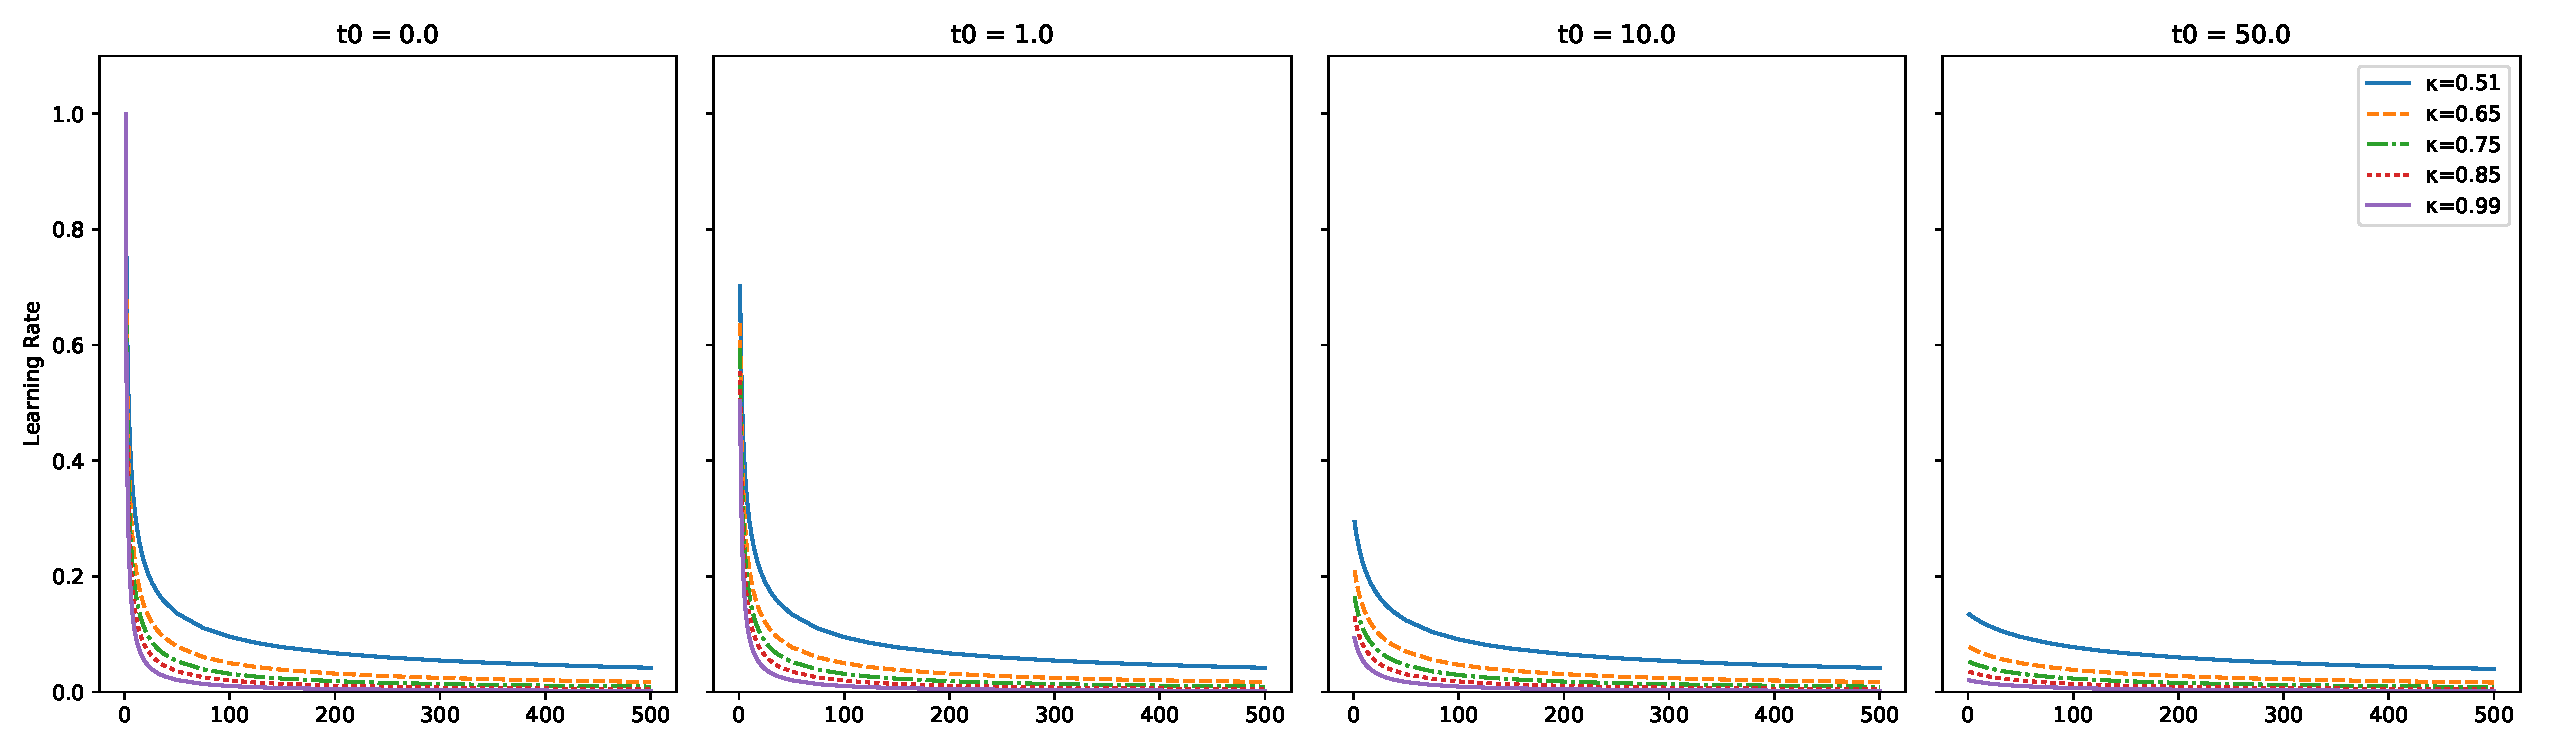
\includegraphics[width=0.97\textwidth]{../Chap1/plots/learning_rate.pdf}
  \caption{Evolution of learning Rates for different values of $\kappa$ and $t_0$ as the number of iterations increases}
  \label{fig:learning-rates}
\end{figure}

While a step size of $\rho_t = \oneover{t}$ meets these criteria, typically\cite{Gopalan2013}\cite{Hoffman2012}\cite{Hoffman2010} the form $\rho_t = (t + t_0)^{-\kappa}$ is used instead, where $t_0 > 0$ is a delay parameter and $\kappa \in (0.5,1]$ controls how quickly the step-size diminishes. Figure \ref{fig:learning-rates} shows how these affect the learning rate over several iterations.

Alternatively one can adapt the learning rate according to instantaneous evaluations of the model fit. In \cite{Amari1998} the step-size was adjusted based on the probability of the data at each step
\begin{align}
\rho_{t+1} & \leftarrow  \rho_t \exp\left( \alpha\beta f^t(\varparam)  - \alpha\rho_t \right) & f^t(\varparam) &= -\elbot{t}
\end{align}
Where  $\alpha$ and $\beta$ are positive constants. Smaller values of $\elbot{t}$ lead to larger step-sizes. Alternatively one can use an estimate of the variance of the gradient\cite{Ho2012} to determine the step-size. Denoting the gradient at time-step t as $g_t$ the algorithm is
\begin{align}
%\begin{split}
\ex{g_t}{} & \approx \bar{g}_t = (1 - \inv{\tau_t})\bar{g}_t + \inv{\tau_t}g_t 
& \rho_t & = \frac{\bar{g}_t \T \bar{g}_t}{\bar{h}_t} \\
\ex{g_t \T g_t}{} & \approx \bar{h}_t = (1 - \inv{\tau_t})\bar{h}_t + \inv{\tau_t}g_t\T g_t &
\tau_{t+1} & = \tau_t(1 - \rho_t) + 1
%\end{split}
\end{align}

\subsubsection*{Stochastic Gradient Descent}
The approach outlined thus far involves evaluating the gradient over the \emph{entire} dataset, which is costly. Instead we consider replacing the gradient with a random function $g \sim G$ such that 
\begin{align}
\ex{g(\varparam)}{G} = \nabla_\varparam \elbo
\end{align}
and therefore replace our deterministic update with a stochastic update at each time-step
\begin{align}
\varparam^{t+1} & \leftarrow \varparam^t + \rho_t g_t(\varparam)
\end{align}

The remaining problem therefore is to sample $g_t(\varparam)$. First note that due to our assumption of exchangeability the gradient will decompose into a sum of terms
\begin{align}
\nabla_\varparam \elbo
& = \nabla_\varparam \ln p(\param | \vv{\beta}) + \nabla_\varparam \ent{\param} + \sum_d \nabla_\varparam \ln p(\xd, \zd | \param, \vv{\alpha}) \\
& = \nabla_\varparam \ln p(\param | \vv{\beta}) + \nabla_\varparam \ent{\param} + \sum_d \nabla_\varparam l_d(\xd; \param) \label{eqn:chap1:sgd-target}
\end{align}

Our approximation focuses on the third summand of \eqref{eqn:chap1:sgd-target}. We can show that this is equivalent to the expected value of $D$ times the per-datapoint gradient according to the empirical distribution of the data $\hat{p}(\vv{x}) = \oneover{D}\sum_d \delta(\vv{x}, \xd)$: 

\begin{align}
\ex{D \text{ } \nabla_\varparam l_d(\vv{x}; \param)}{}
& = \sum_d D \text{ } \nabla_\varparam l_d(\xd, \param) \hat{p}(\xd) \\
& = \sum_d D \text{ } \nabla_\varparam l_d(\xd; \param) \left(\frac{1}{D} \sum_p \delta(\xd, \vv{x}_p)\right) \\ 
& = \sum_d \nabla_\varparam l_d(\xd; \param)
\end{align}

We can approximate this expectation by sampling S datapoints $\vv{x}_s$ at random from the empirical distribution $\hat{p}(\vv{x})$ and then taking the average:
\begin{align}
g(\varparam) = \nabla_\varparam \ln p(\param | \vv{\beta}) + \nabla_\varparam \ent{\param} + \frac{D}{S} \sum_s \nabla_\varparam l_d(\vv{x}_s; \param)
\end{align}
The number of samples, $S$ is called the \emph{minibatch} size. Using several data samples, instead of just one, reduces the variance of the gradient. At the same time, by not using the exact gradient, the residual noise may help the algorithm escape local minima in the negative ELBO\cite{Bottou2004}.

An interesting feature of stochastic gradient descent is that while it is guaranteed to converge, unlike batch gradient descent, its rate of convergence is not dependent on either the initial value or the number of datapoints, and so does not necessarily require a full traversal of the dataset\cite{Bottou2008}. This distinguishes SGD from both batch variational learning and Markov-Chain Monte-Carlo (MCMC) methods both of which require at least several full traversals of the dataset.

That notwithstanding the algorithm does require the total number of datapoints to calculate the approximate gradient and empirical experiments have shown\cite{Broderick2013} that the predictive likelihood of models trained using SGD is adversely affected by incorrect values of $D$. This may not be feasible when using massive datasets, so alternatives such \emph{streaming variational Bayes}\cite{Broderick2013} have been proposed instead.


\subsubsection*{Sampling for Unbalanced Datasets}
While we have presented this in the case of large datasets, stochastic gradient descent is also useful for unbalanced prediction problems. In cases where the number negative datapoints $D^-$ vastly outnumbers the number of positive datapoints $D^+$, it is possible to develop a \emph{weighted} stochastic gradient algorithm such that relatively few negative datapoints are visited, without breaking the convergence guarantees. 

As an example, consider a sampling distribution $q(x)$ such that with some very small probability $\epsilon$ we choose one of the $D^-$ negative datapoints, and with high probability $1 - \epsilon$ we choose one of the $D^+$ positive datapoints. Using the same derivation as importance sampling we can re-write our expectation as

\begin{align}
\ex{D f(\vv{x})}{\hat{p}} \quad
&= \quad \sum_d D f(\xd) \frac{\hat{p}(\xd)}{q(\xd)} q(\xd) 
& = \quad & \ex{D f(\vv{s}) \frac{\hat{p}(\vv{x})}{q(\vv{x})}}{q} \\
& & \approx & \frac{D}{S} \sum_s f(\vv{x}_s) \frac{\hat{p}(\vv{x}_s)}{q(\vv{x}_s)} \\
& & = & \frac{1}{S} \sum_s \frac{f(\vv{x}_s)}{q(\vv{x}_s)}
\end{align}
Where samples $\vv{x}_s$ are drawn from $q(\vv{x})$ and since we assume there are no duplicates in the dataset $p(x) = \oneover{D}$. If $\vv{x}_s$ is sampled from the negative samples, its weight $\oneover{q(x_s)}$ will be the large number $\frac{D^-}{\epsilon}$, whereas if it's sampled from the positive group its weight will be the much smaller $\frac{D^+}{1 - \epsilon}$, up-weighting rarely visited data-points. This method was considerably extended in \cite{Gopalan2013b} (see supplemental material) for the problem of predicting citations within an academic corpus, where the majority of node-pairs had no links between them.



\subsection*{The Natural Gradient}
The gradient can be expressed as\cite{Hoffman2012}:
\begin{align}
\nabla_\varparam f(\varparam) = \lim_{\epsilon \rightarrow 0} \arg \max_{d\varparam} f(\varparam + d\varparam) \qquad \text{where } ||d\varparam||^2 < \epsilon \label{eqn:chap1:euclidean-gradient}
\end{align}
which incorporates the Euclidean distance between parameter values $\varparam$, $d\varparam$.

This distance is not appropriate when comparing probability distributions. Consider the Gaussian distributions $\nor{0}{10000}$ and $\nor{10}{10000}$. These have a considerable degree of overlap, and the Euclidean distance between their parameter-vectors $\left(0, 10000\right)$ and $\left(10, 10000\right)$ is 10, yet the distributions $\nor{0.1}{0.001}$ and $\nor{0}{0.001}$ which have almost no overlap at all, are considered much closer, having a Euclidean distance of 0.1. 

We can instead calculate the gradient in a Riemannian space which respects the information geometry involved by replacing the Euclidean distance $||d\varparam||^2$ with a permuted distance $d\varparam\T G(\varparam) d\varparam$, in which simple algebra\cite{Amari1998} shows that the new gradient update is given by $\inv{G}(\varparam)\nabla_\varparam\elbo$

All that remains is to define a proper distance metric for probability distributions. Setting the $G(\varparam)$ to be the Fisher information of $-\elbo$ is equivalent\cite{Hoffman2012} to minimising the symmetrised KL-divergence between the two distribution parameterisations.

\begin{align}
\symmkl{\varparam}{\varparam'}
 = \ex{\ln \frac{p(x; \varparam)}{p(x; \varparam'}}{\varparam}
 + \ex{\ln \frac{p(x; \varparam')}{p(x; \varparam}}{\varparam'}
\end{align}
and gives rise to the \emph{natural gradient}\cite{Amari1998}. 

The use of the natural gradient can be motivated in other ways. For convex problems batch gradient descent has convergence linear in the number of time-steps\cite{DennisSchnabel1996}. Algorithms can obtain super-linear performance if they add in second-order information\cite{Bottou2004}, by incorporating a positive semi-definite matrix $\hat{H}(\varparam)$ which approximates the Hessian of the objective $\nabla_\varparam \nabla_\varparam -\elbo$.

\begin{align}
\varparam \leftarrow \varparam + \rho_t \inv{\hat{H}}\nabla_\varparam \elbo
\end{align}
Such algorithms include Newton's method, Conjugate Gradient and BFGS. In the case of probability distributions, our target is the log-likelihood $\ln p(\xdat|\param)$, and the Fisher information can, under certain conditions, be represented as the Hessian of that log-likelihood
\begin{align}
G(\varparam) = \int -\nabla_\varparam \nabla_\varparam \ln p(x|\varparam) p(x|\varparam) dx
\end{align}
As the parameter $\varparam$ approaches the optimum, $p(x|\varparam)$ resembles the true data-generating distribution $P(x)$, and so the Fisher information approximates the expected loss (i.e. negative log-likelihood)  $\nabla_\varparam\nabla_\varparam\ex{-\ln p(x|\varparam)}{P(x)}$, making it asymptotically behave like a second order model.


\subsubsection*{Example: Online Latent Dirichlet Allocation}

Our setting is Latent Dirichlet Allocation which was presented on page \pageref{sec:chap1:lda}. For the purposes of later comparisons, we amend the inference procedure outlined there and make $\param$ a random variable, rather than a parameter. Using the standard mean-field variational inference machinery, its approximate posterior distribution in the batch variational setting is given by

\begin{align}
q(\param_k) = \dir{\vv{\beta} + \sum_d \sum_n \vv{w}_{dn} \ex{\zdnk}{q}}
\end{align}
The remaining posteriors remain the same. 

In the case of an online algorithm, the updates for $\thd$ and $\zdnk$ can be thought of as the ``local" E-Step updates, so we need only perform a gradient step for the vocabularies $\Phi = \{ \param_k \}_{k=1}^K$. The gradient of the per-document ELBO with respect to $\varparam_k$, the parameter of the approximate variational Dirichlet posterior for $\param_k$ is given by

\begin{align}
\frac{\delta}{\delta \lambda_{kv}} &\ex{\ln p(\wdoc,\zd, \thd|\param) + \ln p(\param_k)}{q} + \ent{\param_k} \\
& = 
    \sum_v \frac{\delta\text{ } \ex{\ln p(\param_{kv})}{q}}{\delta \lambda_{kt}} 
    \left( 
        -\frac{\lambda_{kt}}{D}
        +\frac{\beta_{kt}}{D}
        +\sum_n w_{dnv}\ex{\zdnk}{q}
    \right)\\
& = 
    \sum_v -\frac{\delta^2 \text{ } \ex{\ln q(\param_k)}{q}}{\delta \lambda_{kt} \delta \lambda_{kv}} 
    \left( 
        -\frac{\lambda_{kt}}{D}
        +\frac{\beta_{kt}}{D}
        +\sum_n w_{dnv}\ex{\zdnk}{q}
    \right) \label{eqn:chap1:fisher-in-grad}
\end{align}
where in equation \eqref{eqn:chap1:fisher-in-grad} we use the fact that $\ex{\ln p(\param_k)}{q}$ is the derivative of the log-normaliser of $q(\param_k)$. This second-order derivative is the Fisher information for $q(\param_k)$, so the natural gradient is just the second term in the product. Obtaining the natural gradient, by pre-mupltiplying by the inverse of the Fisher information and then scaling it by $\rho_t D$ leads to the stochastic gradient-update for $\varparam$

\begin{align}
\varparam^{t+1} \leftarrow (1-\rho_t) \varparam^t + \rho_t \left( 
        \vv{\beta}
        + D \sum_n w_{dnv}\ex{\zdnk}{q}
    \right)
\end{align} 
If we use a minibatching the scaling term $D$ is replaced with $\frac{D}{S}$. It is interesting to note that in the case where $D = S$ the equation for the natural gradient is identical to the parameter of the posterior distribution obtained via the batch method. This was first described in \cite{Sato2001}, which showed that in the variational EM setting, where there is a single global parameter $\param$ in the exponential family, that the batch update is equivalent to doing a natural gradient update on the entire dataset. This result was later extended\cite{Hoffman2012} to include multiple global variables with exponential-family distributions. This insight means that natural gradient methods can be be obtained without explicitly determining the Fisher information matrix for the conjugate posteriors of exponentially-distributed random variables.

Variants of this online-learning algorithm exist. In one case\cite{Mimno2012a} the model was partially Rao-Blackwellised, by analytically integrating out $\thd$. A Gibbs sampler was then used to infer \emph{sparse} values for $\zdnk$ in the ``local" step, and these were were then used to update the vocabulary parameters $\param_k$ in a gradient step. As well as the computational benefits of being able to use sparse computations throughout, this also helped convergence by relaxing the mean-field independence assumptions. A similar relaxation of the independence assumption has also been employed\cite{Hoffman2015} using the structured variational posterior \\
$q(\zdat, \Theta, \Phi) = \prod_k q(\param_k)\prod_d q(\thd, \vv{z}_d | \param)$. Other work on stochastic gradient descent has included the use of Langevin Dynamics\cite{Welling2011} which adds zero-mean Gaussian noise with isotropic variance equal to $\rho_t I$ to the stochastic estimate of the gradient at each timestep.%, and Riemannian Langevin Dynamics\cite{Patterson2013} which adds noise $\vv{epsilon}_t \sim \nor{0}{\rho_t G(\varparam)}$ to a modified stochastic estimate of  the \emph{natural} gradient, where $G(\varparam)$ is the Fisher information as before.



\section{Non-Parametric Bayesian Priors}
\label{sec:chap1:DPs}
Determining the number of components is an issue with mixture and admixture models. A simple approach is to try different counts and evaluate the fit on held-out data. This can be combined with heuristic methods such as canopy-clustering\cite{McCallum2000} to determine an appropriate range of component-counts  in advance.

Thus far we have used a Dirichlet prior distribution over our topics. While we have noted that draws from a Dirichlet distribution are on the simplex, they can also be thought of as PMFs.

This Dirichlet can be parameterised to encode a preference for sparse topic counts by specifying small hyperparamters (see figure \ref{fig:dirichlet-params}). The mechanism is more obvious if one considers the two-parameter definition of a Dirichlet distribution (used in \cite{MacKay1995}\cite{Wallach2006}\cite{Wallach2009a} among others), where one writes $\vv{\theta} \sim \dir{\alpha \vv{m}}$ where $\vv{m}$ is the ``base-measure" on the simplex, and $\alpha$ is a ``concentration" parameter. This reflects the fact that two Dirichlet distributions may represent the distribution (e.g. $(2, 6, 10, 4)$ and $(0.2, 0.6, 1, 0.4)$) which differ only in ``concentration", i.e. by how much will a single observation affect the posterior. Small concentration values encode preferences for sparser models.

An interesting property of the Dirichlet is its aggregation property: given a Dirichlet distribution over a $K-1$ simplex parameterised by $\vv{\alpha}$, one can derive a Dirichlet distribution over a smaller $J-1$:
\begin{equation}
\left(
    \sum_{i \in A_1} \param_i, \ldots, \sum_{i \in A_J} \param_i
\right)
\sim
\dir{
    \sum_{i \in A_1} \alpha_i, \ldots, \sum_{i \in A_J} \alpha_i
}
\end{equation}
To prove this property, note first that one can draw a sample $\param \sim \dir{\vv{\alpha}}$ by drawing multiple samples $z_k \sim \Gamma(\alpha_k, 1)$ and setting $\param = \oneover{\sum_k z_k} \vv{z}$. This can be verified using the standard change-of-variable formula. Hence
\begin{align}
\begin{split}
\left(
    \sum_{i \in A_1} \param_i, \ldots, \sum_{i \in A_J} \param_i 
\right)
& = 
\oneover{\sum_k z_k}
\left(
    \sum_{i \in A_1} z_i, \ldots, \sum_{i \in A_J} z_i
\right) \\& \sim
\oneover{\sum_k \gam{\alpha_k}{1}}
\left(
    \sum_{i \in A_1} \gam{\alpha_i}{1}, \ldots, \sum_{i \in A_J} \gam{\alpha_i}{1}
\right) \\
& \sim
\dir{
    \sum_{i \in A_1} \alpha_i, \ldots, \sum_{i \in A_J} \alpha_i
}
\end{split}
\end{align}


\newcommand \eventspace { \mathcal{X}  }
\newcommand \sigalgebra { \mathcal{B}  }

Denote by $\eventspace$ the event-space, and by $\sigalgebra$ a $\sigma$-algebra defined on that set: which is to say, first, a set such that $\eventspace \in \sigalgebra$; second, that if $B \in \sigalgebra$ its complement $B^{C} \in \sigalgebra$ and third, that for every countable collection of sets in $\sigalgebra$, $\{ B_i \}_{i=1}^{\infty}$, its union is also in $U_{i=1}^{\infty} B_i \in \sigalgebra$. A function $\mu : \eventspace \rightarrow [0, \infty]$ is called a measure if it is countably additive and $\mu( \emptyset ) = 0$. The triple $(\eventspace, \sigalgebra, \mu)$ defines a measureable space. If $\mu(\eventspace) = 1$ then the measure is a probability measure.

The Dirichlet Process (DP) is a measure over all possible probability measures on $(\eventspace, \sigalgebra)$. We write $G \sim \DP{\alpha, H}$ if any \emph{finite} partition of $\eventspace$ has a Dirichlet distribution\cite{Ferguson1973} :

\begin{align}
\left(
    G(\cup_{i \in A_1} B_i),
    \ldots,
    G(\cup_{i \in A_K} B_i)
\right)
\sim
\dir{
    \left(
        \alpha H(\cup_{i \in A_1} B_i),
        \ldots,
        \alpha H(\cup_{i \in A_K} B_i)
    \right)
}
\end{align}
where $\alpha > 0$ is the concentration parameter and $H$ is the base-measure on the event-space. \fixme{Kolmogorov}. As draws from the DP are discrete, one can write the distribution as

\bflong{Check this}

\begin{equation}
G = \sum_{k=1}^{\infty} \theta_k \delta_{\phi^*_k} \label{eqn:ch1:dp-as-weighted-atoms}
\end{equation}
where $\delta$ is the dirac-delta, $\phi^*_k$ is an atom\footnote{In a $\sigma$-algebra $\sigalgebra$ a set $B \in \sigalgebra$ is an atom if for any strict subset $B' \subset B$ its measure $\mu(B') = 0$. We denote by $\phi_i \sim G$ the $i$-th draw from a DP $G$, and by $\phi^*_k$ the $k$-th \emph{distinct} draw from that DP} and $\theta_k$ is its corresponding probability. Draws from the DP follow in the usual manner
\begin{align}
\phi_i|G & \sim G &
\phi_i|\phi_1,\ldots,\phi_{i-1},G & \sim G &
G \sim \DP{\alpha, H}
\end{align}
If one marginalises out G entirely one obtains the following marginal and conditional distributions, which follow a P\'olya Urn scheme\cite{Blackwell1973}
\begin{align}
\phi_i &
\sim H &
\phi_i | \phi_1, \ldots \phi_{i-1} &
\sim \frac{\sum_{j=1}^{i-1} \delta_{\phi_j} + \alpha H}{i + \alpha - 1}
\end{align}
If one denotes by $n^i_k = \sum_{j=1}^{i-1} \one_{\phi_i = \phi^*_k}$ the number of times the distinct atom $\phi^*_k$ has been observed, this can be re-written to given the standard Chinese restaurant process (CRP)\cite{Neal2000}, in which the table $z_i$ at which customer $i$ is sat is either an existing table $k$ with probability proportional to the number of customers already sat there, or a new table with probability $\frac{\alpha}{i + \alpha - 1}$
\begin{align}
p(z_i = k) & = \frac{n^i_k + \alpha}{i + \alpha - 1} &
p(z_i = K + 1) & = \frac{\alpha}{i + \alpha - 1}
\end{align}
The corresponding distinct atom at table k is directly sampled from the base measure $\phi^*_k \sim H$. Note that this exhibits a ``rich-get-richer" property in which the more customers are sat at a table, the greater the probability that a new customer will be sat at that table.

This arrangement of observations -- or ``customers" --  at tables is a partitioning of a potentially infinite stream of exchangeable observations into an infinite sequence of tables, each associated with a distinct atom $\phi^*_k$, which it should be clear is equivalent to a clustering. In the presence of finite data only a finite number of tables employed.

\bflong{Add note about Dirichlet dir stick breaking}

An alternative to the CRP is the stick-breaking process\cite{Sethuraman1994}. Whereas the CRP is concerned with the assignment of observations to partitions, the stick-breaking process, is concerned with the estimation of the size of the partitions, from largest to smallest: this is the problem of estimating $\theta_k$ in \eqref{eqn:ch1:dp-as-weighted-atoms}. This proceeds by recursively using draws from a Beta distribution to assign to proportion of the remaining probability mass to each distinct atom. Given a dirichlet process $\DP{\alpha, H}$ one makes draws $\vv{\theta} \sim \DP{\alpha, H}$ by

\begin{align}
\theta_k & = u_k \prod_{j=1}^{k-1} (1 - u_j) &
u_k & \sim \betadist{1}{\alpha} &
\phi^*_k \sim H
\end{align}


\subsubsection*{Example: Infinite Mixture of Multinomials}
On page \pageref{sec:ch1:mom} we introduced the mixture of multinomials, using the EM algorithm. Denoting by $H$ the prior distribution on the topic vocabularies, $\dir{\vv{\beta}}$, and using a symmetric prior for the mixture components $\dir{\alpha \one}$ the finite mixture of multinomials is
\begin{align}
\vv{\theta} & \sim \dir{\alpha \one} &
\zd|\vv{\theta} & \sim \muln{\vv{\theta}}{1} & 
\xd|\zd, \params & \sim \muln{\param_{z_{d}}}{1} & 
\param_k|H & \sim H
\end{align}
By letting $G = \sum_k^\infty \theta_k \delta_{\vv{\phi}^*_k}$ we can re-write this as an infinite mixture\cite{Antoniak1974} of multinomials using the Dirichlet Process.

\begin{figure}
\centering
    \subfigure[]{
        \resizebox{0.40\textwidth}{0.40\textwidth}{
            %\documentclass{standalone}
%\usepackage{tikz}
%\usepackage{xcolor}
%\usetikzlibrary{fit,positioning}
%
%\usepackage{amsmath}
%\usepackage{amssymb}
%\usepackage{amsfonts}
%\usepackage{mathtools}
%\usepackage{graphicx}
%
%\begin{document}

% ---------------------------------------------------
% Comment above for inclusion in other docs
% ---------------------------------------------------

\begin{tikzpicture}
\coordinate (alpha)   at (0,2);
\node (alpha) at (2,4) [circle, draw, inner sep=1pt, fill, label=above:$\alpha$] { };
\node (theta) at (2,2) [circle, draw, text width = 16pt] {$\text{ }u_k$};

\node (b) at (4,4) [circle, draw, text width = 16pt] {$\text{ }H$};
%\node (b) at (2,2) [circle, draw, inner sep=1pt, fill, label=above:$\beta$] { };
\node (z) at (2,0) [circle, draw, text width = 16pt] {$z_d$};

\node (psis) at (4,2) [circle, draw] {$\phi^*_k$};
\node (w) at (4,0) [circle, draw, text width = 16pt, fill=gray!50] {$w_{dn}$};

 
\draw[->] (alpha) -- (theta);
\draw[->] (b.south) -- (psis.north);
 
\draw[->] (theta.south) -- (z.north);
\draw[->] (z.east) -- (w.west);
\draw[->] (psis) -- (w);
 
\draw (1,-.7) rectangle (6.,1);
\draw (3,-.6) rectangle (5,.75);
\draw (1,1.4) rectangle (5,2.6);
 
\node at (5.5,-.5) {$D$};
\node at (4.8,-.3) {$N$};
\node at (4.8,1.6) {$\infty$};
  
\end{tikzpicture}

% ---------------------------------------------------
% Comment below for inclusion in other docs
% ---------------------------------------------------

%\end{document}
        }
    }
    \subfigure[]{
        \resizebox{0.55\textwidth}{0.40\textwidth}{
            %\documentclass{standalone}
%\usepackage{amsmath}
%\usepackage{tikz}
%\usepackage{xcolor}
%\usetikzlibrary{fit,positioning}
%\begin{document}

% ---------------------------------------------------
% Comment above for inclusion in other docs
% ---------------------------------------------------


\begin{tikzpicture}

\coordinate (alpha_zero)   at (0,2);
\node (alpha_zero) at (2,4) [circle, draw, inner sep=1pt, fill, label=above:$\alpha$] { };
\node (theta_zero) at (2,2) [circle, draw, text width = 16pt] {$\text{ }u_{0k}$};

\coordinate (alpha)   at (0,0);
\node (alpha) at (0,0) [circle, draw, inner sep=1pt, fill, label=above:$\gamma$] { };
\node (theta) at (2,0) [circle, draw, text width = 16pt] {$\text{ }u_{dk}$};

\node (b) at (6,4) [circle, draw, text width = 16pt] {$\text{ }H$};
\node (z) at (4,0) [circle, draw, text width = 16pt] {$z_{dn}$};

\node (psis) at (6,2) [circle, draw] {$\phi_k$};
\node (w) at (6,0) [circle, draw, text width = 16pt, fill=gray!50] {$w_{dn}$};

 
\draw[->] (alpha_zero) -- (theta_zero);
\draw[->] (theta_zero.south) -- (theta.north);
\draw[->] (alpha) -- (theta);
\draw[->] (b.south) -- (psis.north);
 
\draw[->] (theta.east) -- (z.west);
\draw[->] (z.east) -- (w.west);
\draw[->] (psis) -- (w);
 
%\draw (1.3,-.7) rectangle (8.,1);
%\draw (3,-.6) rectangle (7,.75);
%\draw (5.2,1.4) rectangle (6.8,2.6);
% 
%\node at (7.5,-.5) {$D$};
%\node at (6.8,-.3) {$N$};
%\node at (6.5,1.6) {$\infty$};

\draw (1.2,-.7) rectangle (7.5,1);
\draw (3,-.6) rectangle (7,.75);

\draw (1.,-0.9) -- (1.,2.6) -- (7,2.6) -- (7,1.4) -- (2.8,1.4) -- (2.8, 0-.9) -- (1., -0.9);

 
\node at (7.3,-.5) {$D$};
\node at (6.75,-.4) {$N$};
\node at (6.75,1.6) {$\infty$};
  
\end{tikzpicture}

% ---------------------------------------------------
% Comment below for inclusion in other docs
% ---------------------------------------------------

%\end{document}
        }
    }

    \caption{Plate diagrams for (a) an infinite mixture of multinomials and (b) an infinite admixture of multinomials (``Hierarchical Dirichlet Process")} using the stick-breaking construction.
\label{fig:inf-plates}
\end{figure}

\begin{align}
G|\alpha, H & \sim \DP{\alpha, H} &
\phi_d|G & \sim G &
w_{dn}|\phi_d & \sim \muln{\phi_d}{1}
\end{align}
Rewriting this using a stick-breaking construction one obtains the model shown in figure \ref{fig:inf-plates}.
\begin{align}
\theta_k & = u_k \prod_{j=1}^{k-1} (1-u_j) &
u_k & \sim \betadist{1}{\alpha} &
\phi^*_k & \sim \dir{\vv{\beta}} \\ 
z_d & \sim \muln{\vv{\theta}}{1} &
w_{dn} & \sim \muln{\vv{\phi^*_{z_d}}}{1}
\end{align}
Using a mean-field approximation, the variational posterior is $q(\vv{\Phi^*}, \vv{u}, Z) = \prod_k^{T_K - 1} q(u_k) \prod_k^{T_K}q(\phi^*_k) \prod_d q(z_d)$. This approximation \emph{truncates} the space of the Dirichlet process to some upper limit $T_K$: $q(u_{T_K} = 1) = 1$ and so for any $k > T_K$, $q(z_d = k) = q(z_d > K) = 0$. This leaves $T_K -1$ stick-lengths $u_k$ to estimate.

Given that the number of partitions employed cannot exceed the number of documents, setting $T_K = D$ is reasonable, though in practice the upper-bound on component count can be much smaller. By choosing conjugate distributions for $\phi^*_k$ and $u_k$ and taking derivatives and solving in the usual manner, one obtains the following distributions for the variational posterior factors\cite{Blei2006b}.
\begin{align}
q(u_k) & =
    \betadist{
        1 + \sum_d \ex{z_{dk}}{q}
       }{
           \alpha + \sum_d \sum_{j={k+1}}^{T_K} \ex{z_{dj}}{q}
       } \label{eqn:ch1:inf-mom-var-algor-first}\\
q(z_{dk}) & \propto 
    \ex{\ln u_k}{q} 
    + \sum_{k}^{T_K-1}
        \ex{\ln (1 - u_k)}{q}
        + \ex{\phi^*_k}{q}\top \wdoc
        - \ex{a(\phi^*_k)}{q} \\
q(\phi^*_k) & =
    \dir{
        \vv{\beta} + \sum_d \ex{z_{dk}}{q} \wdoc
    } \label{eqn:ch1:inf-mom-var-algor-first-last}
\end{align}
where $\vv{w}_d$ is a bag-of-words representation of the d-th document.

The likelihood of new documents is approximated by
\begin{align}
p(\vv{w}^* | W, \alpha, \vv{\beta})
    &= \int
        \sum_{k=1}^\infty \theta_k(\vv{u}) p(\vv{w}^* | \vv{\phi}^*_k)
        dP(\vv{u}, \Phi^* | W, \alpha, \vv{\beta}) \\
    &\approx \sum_k^{T_K} \ex{\theta_k(\vv{u})}{q} \ex{p(\vv{w}^* | \vv{\phi}^*_k)}{q}
\end{align}
where $\theta_k(\vv{u}) = u_k \prod_{j=k+1}^\infty (1 - u_j)$.


\subsubsection*{Example: Infinite Admixture of Multinomials}
As with the finite mixture of multinomials, by denoting the Dirichet prior over vocabularies as H, we can define the finite admixture of multinomials as:
\begin{align}
\thd & \sim \dir{\alpha \one} &
\zdn|\thd & \sim \cat{\thd} & 
\xdn|\zdn, \param & \sim \muln{\param_{z_{dn}}}{1} & 
\param_k & \sim H
\end{align}
We can make this model extend to infinite admixtures by using a hierarchy of Dirichlet Processes (HDP)\cite{Teh2006b}. Since draws from the DP are discrete, this allows for the same atoms to be shared in different documents with different probabilities.
\begin{align}
G_0|\alpha, H & \sim \DP{\alpha, H} &
G_d|\gamma, G_0 & \sim \DP{\gamma, G_0} \\
\phi_{dn}|G_d\text{ }\text{ } &\sim G_d &
\xdn|\phi_{dn}\text{ }\text{ } & \sim \muln{\phi_{dn}}{1}
\end{align}
This model can be representing using a hierarchical stick-breaking construction, illustrated in figure \ref{fig:inf-plates}.
\begin{align}
\theta_{0k} & = u_{0k} \prod_{j=1}^{k-1}(1-u_j) &
u_{0k} & \sim \betadist{1}{\alpha} \qquad\qquad
\phi^*_k \sim H \\
\theta_{dk} &= u_{dk} \prod_{j=1}^{k-1}(1 - u_{dj}) &
u_{dk}|\vv{u}_{0} & \sim \betadist{\gamma u_{0k}}{\gamma ( 1 - \sum_{j=1}^{k} u_{0j} )} \\
\zdn | \thd & \sim \muln {\thd}{1} &
\xdn | \zdn, \Phi^* &\sim \muln{\phi^*_{z_{dn}}}{1}
\end{align}
As with the infinite mixture model, one can approximate the true posterior using a truncated, approximate, variational distribution
\begin{equation}
q(\vv{u}_0, U, Z, \Phi^*) = \prod_{k=1}^{T_K} q(\phi^*_k) \left( \prod_{k=1}^{T_K-1} q(u_{0k}) \prod_{d=1}^D q(u_{dk})\right) \prod_{d=1}^{D}\prod_{n=1}^{N_d} q(z_{dn})
\end{equation}
Standard application of the rules of variational inference leads to the following distributions for the approximate posterior's factors
\begin{align}
a = 2
\end{align}
\bflong{Add inference scheme}

Markov-Chain Monte Carlo (MCMC) methods have also been employed for the Dirchlet Processes of course, typically ``collapsing" out $G$ and using the Chinese Restaurant Process to sample assignments for each observations\cite{MacEachern1994}\cite{Escobar1995}\cite{Neal2000}, though truncated stick-breaking methods have also been employed\cite{Ishwaran2001}. Empirical comparisons of infinite mixture inference schemes model using Gibbs sampling via the Chinese Restaurant Process; Gibbs sampling using truncated stick-breaking process; and the variational inference scheme given in equations \eqref{eqn:ch1:inf-mom-var-algor-first}-\eqref{eqn:ch1:inf-mom-var-algor-first-last} have shown that variational methods converge much fastest, but sampling using truncated stick-breaking produces models which best explain held-out observations\cite{Blei2006b}


The HDP, being the non-parametric version of LDA, has like LDA seen a similar degree of interest in inference schemes, which include non-parametric variants of the collapsed CVB/CVB0 algorithsm\cite{Sato2012a}, and and online variational algorithms using natural gradients\cite{Wang2011a}.

\subsubsection{Pitman-Yor Process}
\begin{figure}
  \centering
    \hspace*{-1.5cm}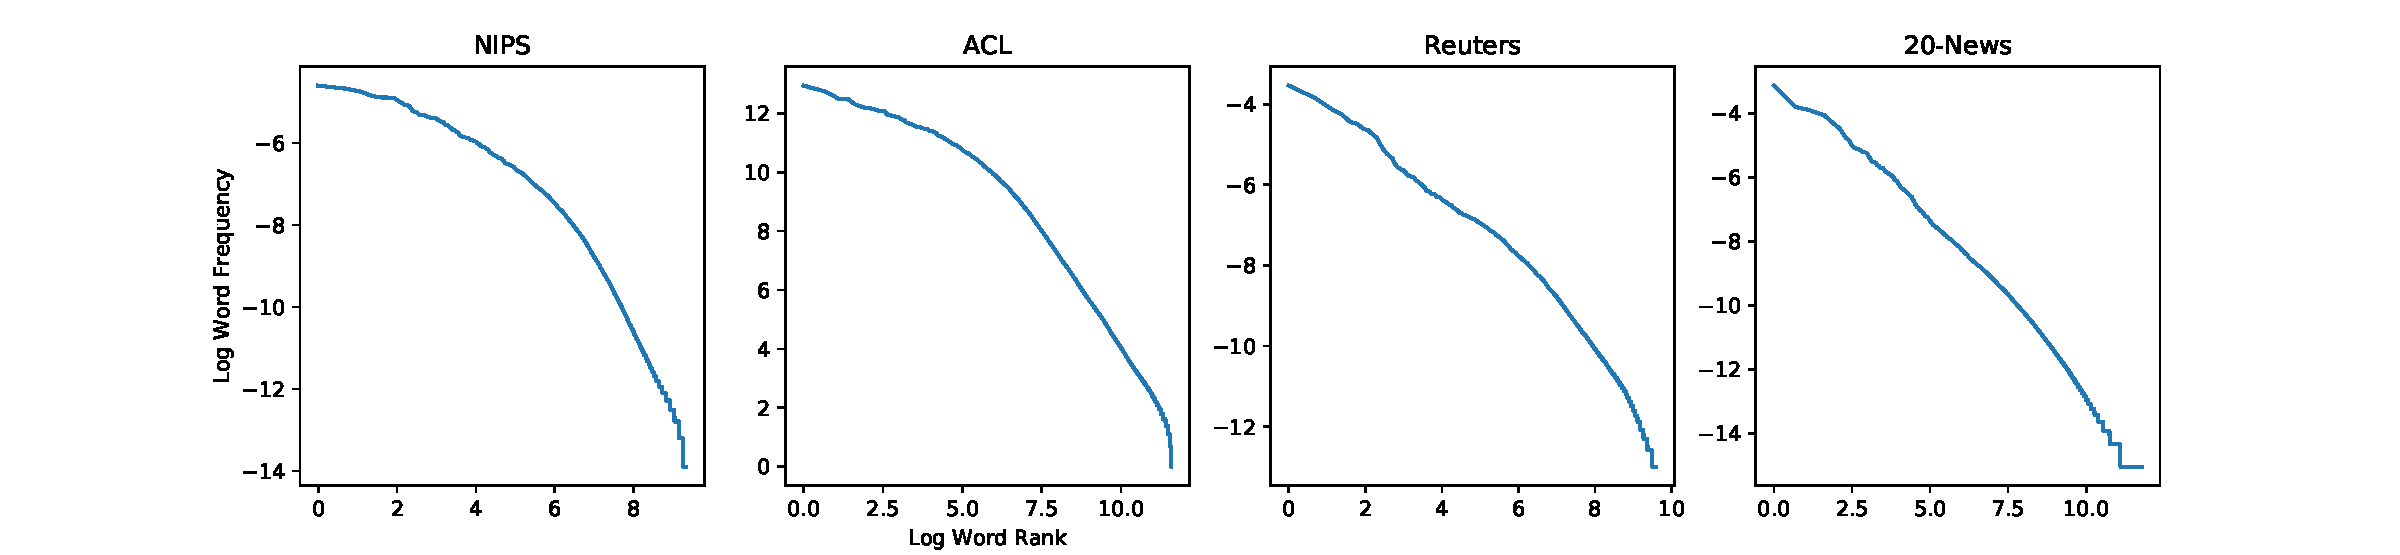
\includegraphics[width=1.25\textwidth]{../Chap1/plots/zipfian_words.pdf}
  \caption{Plot of word-ranks, organised from most to least frequent, on a log-log scale for four datasets: NIPS, the Association for Computational Linguistics (ACL) corpus, Reuters-21378 and 20-News. 20-News has the straight-line common in observations with Zipfian distributions}
  \label{fig:zipfian-words}
\end{figure}
The distribution of words in corpora often follows power-law distribution, sometimes known as the Zipfian distribution in linguistics\cite{Montemurro2000}. Several examples are shown in figure \ref{fig:zipfian-words}. While one can approximate this using hierarchical Dirichlet language models\cite{MacKay1995} it is still not an ideal fit to the data.

Similarly, experiments on the impact of hyper-parameter learning in finite admixture models have shown that the prior distribution of topics itself often exhibits a similar power-law distribution: there are a few topics which are highly likely a priori, then ``long" tail topics that are  much less likely\cite{Wallach2009a}.

The Pitman-Yor Process (PYP), also known as the Two-Parameter Poisson-Dirichlet Process, is an adaptation of the Dirichlet process, over measures which exhibit this power-law behaviour. A PYP is defined by a base measure $H$, a concentration parameter $\alpha > -d$ and a \emph{discount} parameter $0 \leq d < 1$. 

As with the dirichlet process, one can marginalise out the measure drawn from a Pitman-Yor Process and express the probability of draws directly in terms of the hyper-parameters
\begin{align}
\phi_d|G & \sim G &
G & \sim \PYP{d, \alpha, H} \\
\phi^*_k &\sim H &
\phi_n | \phi_1, \ldots, \phi_{n-1} & \sim 
    \frac{\sum_{j=1}^{i-1} \delta_{\phi_j} - d + (\alpha + dK) H}{i + d + \alpha - 1} \label{eqn:ch1:pyp-marginal}
\end{align}
\bflong{This is wrong!}
From this perspective it can be shown that the DP is just a special case of the PYP where the discount parameter $d=0$. If $\alpha = 0$ and $d=\half$ the resulting process is equivalent to an Inverse-G Equation \eqref{eqn:ch1:pyp-marginal} also indicates that the Chinese Restaurant Process can be constructed by incorporating the discount parameter in the probabilities.
\begin{align}
p(z_i = k) & = \frac{n^i_k - d}{i + \alpha - 1} &
p(z_i = K + 1) & = \frac{\alpha + dK}{i + \alpha - 1}
\end{align}
where $K$ indicates the number of ``tables" sat prior to $i$


The stick-breaking construction follows similarly to the DP. Given a Pitman-Yor process $\PYP{d, \alpha, H}$ one makes draws $\vv{\theta} \sim \PYP{d, \alpha, H}$ by

\begin{align}
\theta_k & = u_k \prod_{j=1}^{k-1} (1 - u_j) &
u_k & \sim \betadist{1-d}{\alpha + kd} &
\phi^*_k \sim H
\end{align}
It can be seen that the stick-breaking process representation of the DP is a special case of this more general stick-breaking process where both parameter of the Beta distribution can vary. This general process is known as the GEM distribution\cite{Pitman2002}\bfshort{Everyone cites this paper for this name, but I'm not sure they're doing it right}.

Pitman-Yor processes have been used both as priors over infinite mixtures and admixtures: notably the HDP was extended to use both Pitman-Yor processes for topic-distributions and for for word-distributions\cite{Buntine2014}, where they captured the power-law distribution of words, and admitted a potentially infinite vocabulary.

\subsubsection*{Example: Pitman-Yor Language Model}
On page \pageref{sec:chap1:mackay-lang-model} we discussed the hierarchical Dirichlet language-model. As should be clear now, the Dirichlet distribution is not an ideal fit for words as it does not exhibit a power-law. However by using Pitman-Yor Processes one can capture this aspect of 

The PYP language model\cite{Teh2002}

\bflong{Just do a summary, point to the paper for inference, add note it uses CRP but to consider SeqMem or alternative}


\bflong{Move ref to LDA with PYP-Lang-Model here.}

\bflong{Simplify the discussion of language models and IKN}.




 


%Dirichlet processes, like Dirichlet distributions assume that components are near-independent\footnote{The requirement that samples like on the simplex means they cannot be considered \emph{fully} independent}. The Discrete Infinite Logistic Normal (DILN) distribution\cite{Paisley2012}\cite{Paisley2012b} incorporates a HDP into CTM in order to capture correlations amongst a potentially infinite number of components. The derivation proceeds in several stages. 
%Firstly, one should note that one can implement a HDP using a combination of stick-breaking processes and gamma-processes, the latter analogous to the usual approach for sampling from a (finite) Dirichlet
%\begin{align}
%G_0 & = \sum_{k=1}^\infty \hat{\pi}_k \prod_{j=1}^{k-1} (1 - \hat{\pi}_j)\delta_{\phi_k} & 
%\hat{\pi}_k & \sim \mathcal{B}eta\left(1, \gamma\right) &
%\delta_{\phi_k} & \sim H \\
%G_d|G_0, Z & = \sum_{k=1}^\infty \frac{Z_k^{(d)}}{\sum_{j=1}^\infty Z_j^{(d)}} \delta_{\phi_k} &
%Z_k^{(d)} | G_0 &\sim \gam{\beta \pi_k}{1} &
%\pi_k & = \hat{\pi}_k \prod_{j=1}^{k-1} (1 - \hat{\pi}_j)
%\end{align}
%
%To capture a sense of correlation, each atom $\phi_k$ is associated with a location $\vv{l}_k \in \VReal{d}$, where $d$ is set equal to $K$ for the purposes of inference
%\begin{align}
%G_0 | \gamma, H, L & \sim \DP{\gamma H \times L } &
%G_d^{\text{DP}} | \alpha, G_0 & \sim \DP{\alpha, G_0} \\
%\eta_d(l) & \sim \GP{\vv{m}(l)}{K(l, l')} &
%G_d\left(\{\phi, l\}\right) & \propto G_d^{\text{DP}}\left(\{\phi, l\}\right) \exp\left(\eta_d(l) \right) \\
%\phi_{dn} |G_d &\sim G_d & w_{dn} | \phi_{dn} & \sim F(\phi_{dn})
%\end{align}
%
%Noting that if $y = bx$ for $x \sim \gam{a}{1}$, then $y \sim \gam{a}{b^{-1}}$, we see we can fold in the exponentiated draw from the GP into the Gamma Process, and thus arrive at this model.
%
%\begin{align}
%\hat{\pi}_k & \sim \mathcal{B}\left(1, \gamma\right) &
%\delta_{\phi_k} & \sim H,\quad \delta_{l_k} \sim L \\
%G_0 & = \sum_{k=1}^\infty \hat{\pi}_k \prod_{j=1}^{k-1} (1 - \hat{\pi}_j)\delta_{\phi_k} & 
%\pi_k & = \hat{\pi}_k \prod_{j=1}^{k-1} (1 - \hat{\pi}_j) \\
%G_d|G_0, Z & = \sum_{k=1}^\infty \frac{Z_k^{(d)}}{\sum_{j=1}^\infty Z_j^{(d)}} \delta_{\phi_k, l_k} &
%Z_k^{(d)} | G_0 &\sim \gam{\beta \pi_k}{e^{-\eta_{dk}}} \\
%\eta_{dk} & \sim \GP{\vv{m}}{K} \\
%\phi_{dn} |G_d &\sim G_d & w_{dn} | \phi_{dn} & \sim F(\phi_{dn})
%\end{align}
%
%A variational inference procedure is given in \cite{Paisley2012b} where a truncated Dirichlet was used to model the DP. Rather than learn a kernel function, the kernel (i.e. covariance) matrix was learnt directly from the values of $\eta_{dk}$ using the usual form $K = \frac{1}{D} \sum_d (\vv{\mu}_d - \vv{m})(\vv{\mu}_d - \vv{m}) + \diag{\vv{v}_d}$ where the variational posterior over the location for document d was $q(\vv{\eta}_d) = \nor{\vv{\mu}}{\diag{\vv{v}_d}}$. With regard to variational posterior over location, its parameters are found using gradient descent, where the gradients are
%\begin{align}
%\frac{\delta \mathcal{L}}{\delta \mu_{dk}} & = \lambda_{dk} - \beta \pi_k - K^{-1}_{k,:} \left( \vv{\mu}_d - \vv{m}\right) &
%\frac{\delta \mathcal{L}}{\delta v_{dk}} & = -\half \left( \lambda_{dk} - K^{-1}_{k,k} + \oneover{v_{dk}}\right)
%\end{align}
%and $\lambda_{dk} = \ex{Z_{dk}}{q} \times \ex{\exp(-\eta_{dk})}{q}$, and these expectations follow the usual form for gamma and log-normal distributions respectively. 
%
%A variant of this approach was additionally used in \cite{Virtanen2012a}


\section{Evaluating Model Fit}
\label{sec:chap1:eval}

A number of methods have been proposed to evaluate admixture models. By far the most popular is perplexity, which is defined as the geometric mean of the reciprocals of token likelihoods. Assuming exchangeability of words, the perplexity for a model $\model$ is defined as

\begin{align}
\perplexity{\model} = \sqrt[n_{d}]{\prod_d \prod_n \frac{1}{p(w_{dn}|\model)}} = \exp \left( \frac{-\sum_d \sum_n \ln p(w_{dn}|\model)}{n_{d\cdot\cdot}} \right) \label{eqn:perp_def}
\end{align}

As explained n \cite{Goodman2001} one can consider that a simple model that assigned uniform probability to 100 words would have a perplexity score of 100. The actual distribution, being non-uniform would be significantly \emph{lower}. Perplexity can also be linked to information theory: the log of a perplexity score gives the entropy of the word likelihoods, and as the entropy (base 2) specifies the average number of bits required to encode each word according to Shannon's source-coding theorem, lower perplexity values indicate better compression schemes.

Taking this further, perplexity can be shown to be a special case of the cross-entropy function $\text{H}[p,q]$ where $p(w_{dv})$ is the empirical distribution of the word, $q(w_{dv})$ is the distribution we've inferred (confusingly denoted $p(w_{dn})$ in \eqref{eqn:perp_def}), and we use $e$ as the base and the natural log in the exponent. 

To evaluate perplexity, one needs to determine the probability of a query (i.e. test) set $\WQuery$ given the training set $\WTrain$. Consider an LDA model in which the document-level topic distributions $\thd$ have been marginalised out, leaving a Polya distribution over the latent per-token topic-assignments $\zdn$, parameterised by a prior $\vv{\alpha}$.

\begin{align}
p(\WQuery|\WTrain) = \int p(\WQuery|\Phi, \vv{\alpha})p(\Phi,\vv{\alpha} | \WTrain) d\Phi d\vv{\alpha}
\end{align}

where due to the assumed exchangeability of documents $p(\WQuery|\Phi, \vv{\alpha}) = \prod_ p(\vv{w}_d^{q}|\Phi, \vv{\alpha})$. Leaving aside the first term in the integrand, one can approximate this integral either by substituting in point estimates for $\Phi$ and $\vv{\alpha}$ or sampling from the posterior - the latter being particularly easy in cases where the model parameters have been fit using Gibbs sampling.

The issue that remains however is how to evaluate $p(\vv{w}_d|\Phi, \vv{\alpha})$, which is dependant on the latent variables $\zdnk$. There are a number of ways in which this can be evaluated, of which two have been used frequently in the literature.

The harmonic mean method has been used in\cite{Griffiths2004}\cite{Griffiths2005}\cite{Wallach2006}, all of which performed inference using collapsed Gibbs samplers. The approach is defined as
\begin{align}
\oneover{p(w)} = \sum_z \frac{p(z|w)}{p(w|z)} \approx \oneover{S} \sum_s \oneover{p(w|\samp{z})}
=  \text{HM}\left[ \left\{ p(\vv{w}|\samp{\vv{z}}, \Phi \right\}_{s=1}^{S}  \right]
\end{align}
where HM is the Harmonic Mean and the approximation comes from implementing an importance sampler using the target $p(z|w)$ as the proposal distribution. Implementing this we can see that 

The sampling distribution over $\zdnk$ is given by

\begin{align}
p(z_{dn} = k | \vv{w}_d, \vv{z}_d^{\setminus n}, \Phi, \vv{\alpha}) \propto \phi_{k,{w_{dn}}}\frac{n_{dk\cdot} + \alpha_k}{n_{d\cdot\cdot} + \sum_j \alpha_j}
\end{align}

The second approach is the left-to-right method, which has been used in \cite{Mimno2011} and \cite{Mimno2012a}. By factorising the likelihood as

\begin{align}
p(\vv{w}|\Phi, \vv{\alpha}) & = \prod_n p(w_n | \vv{w}_{<n}, \Phi, \vv{\alpha}) \\
& = \prod_n \sum_{\vv{z}_{<n}} p(w_n, \vv{z}_{<n}| \vv{w}_{<n}, \Phi, \vv{\alpha})
\end{align}
it is possible to approximate the likelihood using a variant a sequential Monte-Carlo, where each particle $p$ iteratively draws samples of $z^{(p)}_{dn'}$ for $n' \in 1 \ldots n_{d\cdot\cdot}$, and uses these samples to evaluate the overall probability of the likelihood. The full algorithm is given in \cite{Wallach2009}.

When the harmonic mean, left-to-right and several other methods including importance sampling and annealed importance sampling where compared in \cite{Wallach2009} it was found that the harmonic mean method tended to ``wildly overestimate" the true likelihood, while the left-to-right method gave the most accurate estimate.

A method of evaluating perplexity which tests the model's predictive power is ``document-completion" which has been used in \cite{Virtanen2012a}\cite{Asuncion2012}\cite{RosenZvi2004} and measure's the model's predictive power. Each document in the test-set is partitioned into two halves\footnote{Given that words are assumed exchangeable within documents, and that long documents may exhibit structure affecting which topics can be inferred where, one can, and indeed should, permute the word order before splitting each document}: an estimation fragment, $\vv{w}_d^{(e)}$, from which a topic distribution is inferred; and an evaluation document, $\vv{w}_d^{(l)}$, whose likelihood given the inferred topic distribution is calculated. Formally writing this as
\begin{align}
p(\vv{w}_d^{(l)}|\vv{w}_d^{(e)}, \Phi, \vv{\alpha}) = \frac{p(\vv{w}_d^{(l)},\vv{w}_d^{(e)} |\Phi, \vv{\alpha})}{p(\vv{w}_d^{(e)}|, \Phi, \vv{\alpha})}
\end{align}

it should be clear that the methods used above can be used to infer both $p(\vv{w}_d^{(e)}|, \Phi, \vv{\alpha})$ and $p(\vv{w}_d^{(l)},\vv{w}_d^{(e)} | \Phi, \vv{\alpha}) = p(\vv{w}_d | \Phi, \vv{\alpha})$. However the most  popular method used in this case is topic-estimation which involves sampling $\vv{z}_d^{(e,s)} \sim p(\vv{z}_n^{(e)} | \vv{w}^{(e)}, \Phi, \vv{\alpha})$ and then evaluating $\vv{\theta}_d^{(e)}$ as

\begin{align}
\theta^{(e,s)}_{dk} = p(k | \vv{z}^{(e,s)}, \vv{\alpha}) = \frac{n^{(e,s)}_{dk\cdot} + \alpha_k}{n^{(e)}_{d\cdot\cdot} + \sum_j \alpha_j}
\end{align}

from which one can then evaluate the probability of the evaluation document:

\begin{align}
p(\vv{w}_d^{(l)}|\vv{w}_d^{(e)}, \Phi, \vv{\alpha}) \approx
\oneover{S} \sum_s \prod_n \sum_k \phi_{k,w^{(l)}_{dn}}\theta_{dk}^{(e,s)}
\end{align}

In practice, particularly with variational approaches, a single point estimate of $\vv{\theta}_d^{(e)}$ is often used instead\cite{Asuncion2012}, though when evaluating document completion \cite{Wallach2009} found that the topic-estimation method, even when implemented via sampling, compared ``poorly" with left-to-right sampling. 

Thus measures of perplexity are highly dependant on how the held-out likelihood is evaluated, which is rarely described well in the literature. Furthermore, many implementors use hard-coded symmetric priors for baseline topic models, even though the performance of topic models is highly sensitive to the configuration of hyper-parameters\cite{Asuncion2012}\cite{Wallach2006}. Consequently is is difficult to compare different measures of perplexity across different models in different publications.

It does not always follow that models with good (i.e. low) perplexity scores are always interpretable. In\cite{Chang2009} human testers were asked to inspect the topic vocabularies generated by different topic models (LDA, CTM and PLSA). In a ``word-intrusion" test they were asked which word, in a list of words belonging to a single topic, was the wrong word from another topic added by the experimenters. In a ``document-intrustion" they were similarly asked to identify the intruded document in a list of document excerpts belonging to a single topic. The CTM model, despite achieving the best perplexity score, faired worst in both of these tasks. 

%In   \cite{Azzopardi2003} it was shown that when using language-models to aid information retrieval, language models with the best perplexity scores did not always lead to the best precision scores. 

In light of this, some more recent publications such as \cite{Li2006}\cite{Wang2007}\cite{Lindsey2012} have used similar intrusion tests via Mechanical Turk to test the performance of their models.

There are metrics which don't rely on the likelihood. The ``topical coherence" metric, introduced in \cite{Mimno2011} and additionally used in \cite{Mimno2012a} addresses the word-intrusion problem. Assume that if a set of words all belong to a single topic, one would them concentrated in documents belonging to that topic, rather than distributed uniformly across all documents and all topics. Therefore letting $D(t)$ be the number of documents where word $t$ occurs at least once, and $D(t,v)$ be the number of documents containing at least one occurrence each of both $t$ and $v$, the coherence metric is defined as
\begin{align}
C(k; V^{(m)}) = \sum_{t \in V^{(m)}_k} \sum_{v \in V^{(m)}_k,  v \neq t} \ln \frac{D(t, v) + 1}{D(v)}
\end{align}
where $V^{(m)}_k$ is the set of the $m$ most probable words in topic $k$, and the addition of $1$ to the numerator is to avoid taking the log of zero. 

%\fixme{Read this some more. Also pointwise mutual info}

The \emph{empirical likelihood} of \cite{Li2006} tests the generative ability of a model. For each test document, this involves using the model to generate, say, 1,000 synthetic documents, deriving an empirical (in this case multinomial) distribution from each document, and then evaluating the average of the probabilities of the test document according to each of these empirical distributions. This has additionally been used in \cite{Doyle2009}\cite{Mimno2008}. In \cite{Wallach2009} it was shown that this method is an approximation to $p(\vv{w}_d|\Phi, \vv{\alpha}) = \int p(\vv{w}_d, \thd | \Phi)p(\thd|\vv{\alpha})d\thd$ using importance sampling with true posterior employed as a proposal distribution. Were the synthetic documents infinitely long, the two methods would be identical. This analogy points to a potential deficiency of this method however, which is that one would expect the variance of an estimate derived from importance sampling to be very high when sampling from high-dimensional distributions: consequently for very high topic-counts (cases with over 200-topic are common) this may not be a reliable estimator.

\subsection*{Evaluation Against Labelled Data}
With labelled data, specified with a 1-of-$L$ labelling $\vv{t}_d$, one may choose to evaluate the model by comparing it to the inferred topics, $\thd \in \VReal{K}$, where $K$ need not necessarily equal $L$. Many metrics exist for this purpose, of which the most well known is the F1-Score, $F_1 = 2 \frac{p \cdot r}{p + r}$, which is the harmonic mean of precision, $p=\frac{TP}{TP+FP}$ and recall, $r=\frac{TP}{TP+FN}$, and $TP, FP, TN, FN$ refer to the true and false positives and negatives respectively.

%In the presence of soft-clustering and multiple labels one can\footnote{See https://facwiki.cs.byu.edu/nlp/images/2/25/ClusterEvaluation.ppt} define an $F_1$ score for a single topic $k$ and a single label $l$ thusly.

Letting \emph{precision} be the ``number of documents in a cluster that belong there", and recall be be ``did all the documents that should be in this cluster make it in" we derive the following:
\begin{align}
p_{kl} & = \frac{n_{kl}}{n_k} = \frac{\sum_d \theta_{dk} t_{dl}}{\sum_d \theta_{dk}}  & r_{kl} & = \frac{n_{kl}}{n_l} = \frac{\sum_d \theta_{dk} t_{dl}}{\sum_d t_{dl}} \label{eqn:myrecall}
\end{align}

where $n_{kl}$ is the number of documents in cluster $k$ which have the label $l$ and $n_k$ is the number of documents in cluster $k$. We can, for a single topic $k$ and a single label $l$ specify the $F_1$ score as $F_1^{(k,l)} = 2 \frac{p_{kl} \cdot {r_{kl}}}{p_{kl} + {r_{kl}}}$

For a single label $l$ one can take the max across topics $F_1^{(l)} = \max_{k \in 1\ldots K} F_1^{(k,l)}$ and then finally describe the entire corpus using a weighted average of label specific $F_1$ scores, with the weights proportional to the number of documents with each label where $D' = \sum_d \sum_l t_{dl}$ is the total number of label instances, to account for the fact that there may be documents with more than one label, and so $D' \geq D$.


\begin{figure}
  \centering
    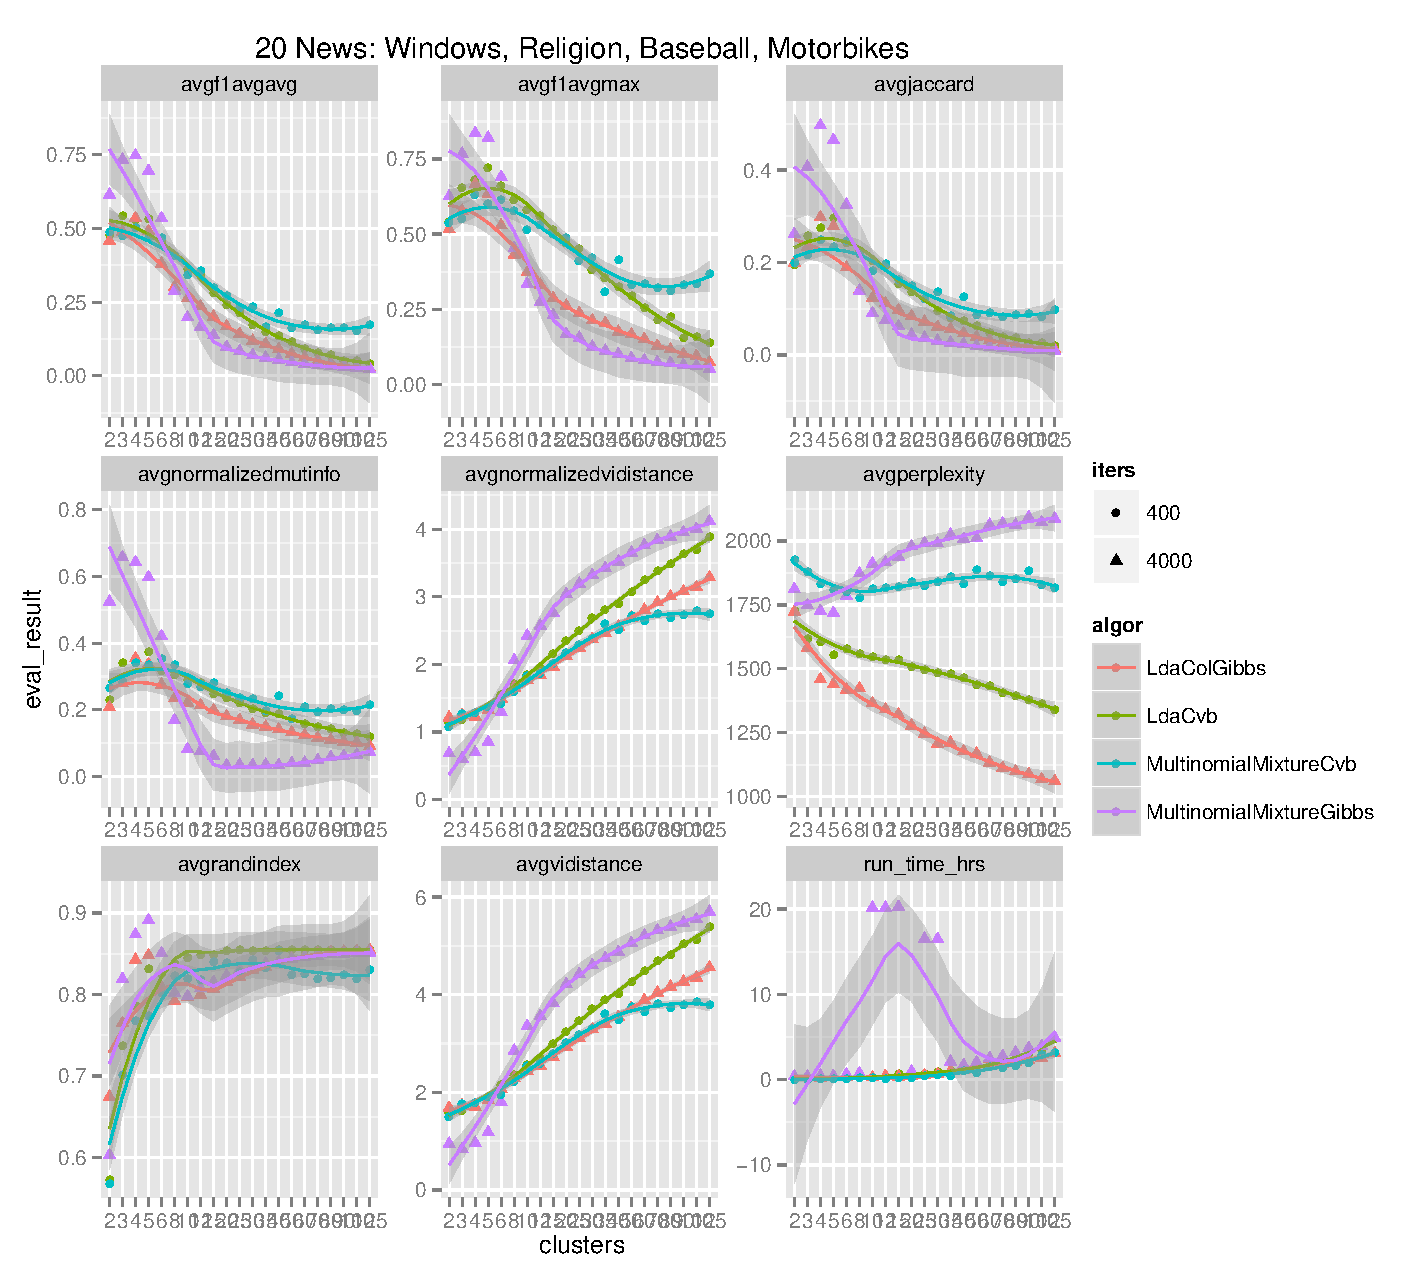
\includegraphics[width=0.9\textwidth]{../Chap3a/plots/20news-2013-03-25.pdf}
  \caption{Results using different accuracy metrics for a mixture of multinomials and LDA on a subset of the 20-news dataset. Trendlines and shading are from a LOESS fit to the points. A variation of the soft F1 measure described in the text is shown where we average over label-specific F1 scores instead of taking the maximum. Held-out likelihood was evaluating using the document-completion metric with inferred topics.}
  \label{fig:eval-metrics-shootout}
\end{figure}


A different approach to comes from the intuition that given two equivalent labelings, one would expect label pairs $z=k$ and $t=l$ to co-occur, and so expect that $p(z,t) \neq p(z)p(t)$, which opens the door to a number of information theoretic measures such as normalised mutual information (NMI) and the Variation of Information (VI) distance..

\newcommand{\TopDist}{\Theta}
\newcommand{\LabDist}{\mathbb{C}}
\newcommand{\NMI}{\text{NMI}}

Given a corpus-wide distribution over topics $\TopDist$ and a corpus wide distribution over labels $\LabDist$ the NMI is defined as a function of the mutual information $\mut{\TopDist}{\LabDist}$

\begin{align}
\NMI & = \frac{\mut{\TopDist}{\LabDist}}{1/2(\ent{\TopDist} + \ent{\LabDist})} &
\mut{\TopDist}{\LabDist} & = \sum_k \sum_l p(\theta_{\cdot k}, t_{\cdot l}) \ln \frac{p(\theta_{\cdot k}, t_{\cdot l})}{p(\theta_{\cdot k})p(t_{\cdot l})}
\end{align}
and the entropies are defined as
\begin{align}
\ent{\TopDist} & = - \sum_k p(\theta_{\cdot k}) \ln (\theta_{\cdot k}) &
\ent{\LabDist} & = - \sum_l p(t_{\cdot l}) \ln p(t_{\cdot l})
\end{align}

In the case of LDA these distributions would be defined as
\begin{align}
p(\theta_{\cdot k}) & =  \frac{1}{D} \sum_d \theta_{dk} ,&
p(t_{\cdot l}) &= \frac{1}{D'} \sum_d t_{dl} ,& 
p(\theta_{\cdot k}, t_{\cdot l}) & = \frac{1}{D'} \sum_d \theta_{dk} t_{dl}
\end{align}
where again $D' = \sum_d \sum_l t_{dl}$ is the total number of label instances, such that $D' \geq D$


The VI distance\cite{Meila2003} is another information-theoretic measure defined over a topic distribution $\TopDist$ and labelling distribution $\LabDist$ as:
\begin{equation}
\dvi{\TopDist}{\LabDist} = \ent{\LabDist} + \ent{\TopDist} - 2 \mut{\LabDist}{\TopDist}.
\end{equation}

$\dvi{\TopDist}{\LabDist}$ is a true metric: it is always non-negative, becomes zero if and only if $\LabDist = \TopDist$, is symmetric, and observes the triangle inequality, $\dvi{X}{Z} + \dvi{Z}{Y} \geq \dvi{X}{Y}$. However the range over which VI distance scores will take is dataset-dependant, and so to compare scores across datasets one can use the \emph{normalized VI distance}\cite{Reichart2009} which is defined as. 

\begin{align}
\text{NVI}\left[ \TopDist, \LabDist \right] = \left\{ \begin{array}{lr}
     \frac{1}{\ent{\TopDist}}\dvi{\TopDist}{\LabDist} & \ent{\TopDist} \neq 0 \\
     \ent{\LabDist} & \text{otherwise}
 \end{array}\right.
\end{align}


The VI distance has been used to compare topics inferred by LDA with manual labelling of over 20,000 news-stories\cite{HeinrichEtAl2005}. 


A well-known metric from the field of clustering is the rand Rand Index, which determines how similar are two ways of partitioning data. It counts fours classes of document-pairs: (a) those which have the same cluster and have the same label; (b) those which have different clusters but share the same label; (c) those which have the same cluster but have different labels; and (d) those which which are not in the same cluster and have different labels.

Given these definitions the index is then $\text{RI} = \frac{a + d}{a + b + c + d}$. This is broadly similar to the idea of accuracy traditionally defined as being $\frac{TP + TN}{TP + FN + FP + TN}$

For the kind of soft-clustering featured in LDA, one would define these counts as
\begin{equation}
\begin{aligned}
a & = \sum_k \sum_{d, {p>d}} \theta_{dk} \theta_{pk} \sum_l t_{dl}t_{pl} & \quad
b & = \sum_k \sum_{d, {p>d}} \theta_{dk} (1 -\theta_{pk}) \sum_l t_{dl}t_{pl}\\
c & = \sum_k \sum_{d, {p>d}} \theta_{dk} \theta_{pk} \sum_{l,m \neq l} t_{dl}t_{ml} & \quad
d & = \sum_k \sum_{d, {p>d}} \theta_{dk} (1- \theta_{pk}) \sum_{l,m \neq l} t_{dl}t_{ml}
\end{aligned}
\end{equation}

Plots of all these metrics, for different topic counts, are given in figure \ref{fig:eval-metrics-shootout} for documents taken from four very different newsgroups from the overall 20-newsgroups dataset.

\section{Experiments}
\label{sec:chap1:experiments}
This is a section

\section{Conclusions}
In this chapter we have introduced the fundamentals of Bayesian inference. We have described the major probabilisitic models used with text: including language-models, mixture-models, and admixture models. In the particular case of admixture models of text, or ``topic models", we have given a cursory overview of the literature. We have demonstrated how admixture models outperform simple mixture models, and how the training scheme affects model fit. 


There is a wealth of information which for reasons of brevity we have not discussed. In the machine learning-literature, it is common to represent text not as vectors of word-counts, but of vectors of word-frequencies, which have been adjusted using words' inverse document-frequencies (to down-weight common stop-words). Standard machine-learning approaches such as K-Means clustering work quite well on this data. In the sense that LDA can be thought of as a matrix factorization approach, in that $W \approx \Theta \Phi$, it has been anticipated by the latent-semantic indexing (or analysis) method, which uses a singular-value decomposition of the TF-IDF matrix. A weakness of this method is that topic ``strengths" may be negative, which difficult to interpret. 

Prior to the publication of LDA, several other methods had been attempted to represent documents as a mixture, of which probabilistic latent-semantic indexing \cite{Hofmann1999a} was the most successful. Unfortunately, like LSI, pLSI used a document indicator variable to associate topic with documents, and so could not generalise to unseen documents. It has been shown\cite{GiKa2003} that LDA is in fact just a proper Bayesian inference scheme for the pLSI. 

The matrix factorisation view of LDA, is also reminiscent of principal components analysis, and in fact a model for principal components analysis generalised to multinomial observations\cite{Buntine2002} published a year before the original LDA paper has been shown to be equivalent to the LDA model: though both were anticipated by an ad-hoc model of chromosome data published in 2000\cite{Pritchard2000}

In chapter two we will discuss further extensions to topic models, using correlation between topics and in chapter three and four we will dicuss how additional observations can be incorporated into topic-models. In chapter five we will use the correlated topic-model framework to consider the problem of predicting inter-document links in a network of academic papers.

\bibliographystyle{plain}
\bibliography{/Users/bryanfeeney/Documents/library.bib}

\end{document}

